\documentclass[twoside]{book}

% Packages required by doxygen
\usepackage{fixltx2e}
\usepackage{calc}
\usepackage{doxygen}
\usepackage[export]{adjustbox} % also loads graphicx
\usepackage{graphicx}
\usepackage[utf8]{inputenc}
\usepackage{makeidx}
\usepackage{multicol}
\usepackage{multirow}
\PassOptionsToPackage{warn}{textcomp}
\usepackage{textcomp}
\usepackage[nointegrals]{wasysym}
\usepackage[table]{xcolor}

% Font selection
\usepackage[T1]{fontenc}
\usepackage[scaled=.90]{helvet}
\usepackage{courier}
\usepackage{amssymb}
\usepackage{sectsty}
\renewcommand{\familydefault}{\sfdefault}
\allsectionsfont{%
  \fontseries{bc}\selectfont%
  \color{darkgray}%
}
\renewcommand{\DoxyLabelFont}{%
  \fontseries{bc}\selectfont%
  \color{darkgray}%
}
\newcommand{\+}{\discretionary{\mbox{\scriptsize$\hookleftarrow$}}{}{}}

% Page & text layout
\usepackage{geometry}
\geometry{%
  a4paper,%
  top=2.5cm,%
  bottom=2.5cm,%
  left=2.5cm,%
  right=2.5cm%
}
\tolerance=750
\hfuzz=15pt
\hbadness=750
\setlength{\emergencystretch}{15pt}
\setlength{\parindent}{0cm}
\setlength{\parskip}{3ex plus 2ex minus 2ex}
\makeatletter
\renewcommand{\paragraph}{%
  \@startsection{paragraph}{4}{0ex}{-1.0ex}{1.0ex}{%
    \normalfont\normalsize\bfseries\SS@parafont%
  }%
}
\renewcommand{\subparagraph}{%
  \@startsection{subparagraph}{5}{0ex}{-1.0ex}{1.0ex}{%
    \normalfont\normalsize\bfseries\SS@subparafont%
  }%
}
\makeatother

% Headers & footers
\usepackage{fancyhdr}
\pagestyle{fancyplain}
\fancyhead[LE]{\fancyplain{}{\bfseries\thepage}}
\fancyhead[CE]{\fancyplain{}{}}
\fancyhead[RE]{\fancyplain{}{\bfseries\leftmark}}
\fancyhead[LO]{\fancyplain{}{\bfseries\rightmark}}
\fancyhead[CO]{\fancyplain{}{}}
\fancyhead[RO]{\fancyplain{}{\bfseries\thepage}}
\fancyfoot[LE]{\fancyplain{}{}}
\fancyfoot[CE]{\fancyplain{}{}}
\fancyfoot[RE]{\fancyplain{}{\bfseries\scriptsize Generated by Doxygen }}
\fancyfoot[LO]{\fancyplain{}{\bfseries\scriptsize Generated by Doxygen }}
\fancyfoot[CO]{\fancyplain{}{}}
\fancyfoot[RO]{\fancyplain{}{}}
\renewcommand{\footrulewidth}{0.4pt}
\renewcommand{\chaptermark}[1]{%
  \markboth{#1}{}%
}
\renewcommand{\sectionmark}[1]{%
  \markright{\thesection\ #1}%
}

% Indices & bibliography
\usepackage{natbib}
\usepackage[titles]{tocloft}
\setcounter{tocdepth}{3}
\setcounter{secnumdepth}{5}
\makeindex

% Hyperlinks (required, but should be loaded last)
\usepackage{ifpdf}
\ifpdf
  \usepackage[pdftex,pagebackref=true]{hyperref}
\else
  \usepackage[ps2pdf,pagebackref=true]{hyperref}
\fi
\hypersetup{%
  colorlinks=true,%
  linkcolor=blue,%
  citecolor=blue,%
  unicode%
}

% Custom commands
\newcommand{\clearemptydoublepage}{%
  \newpage{\pagestyle{empty}\cleardoublepage}%
}

\usepackage{caption}
\captionsetup{labelsep=space,justification=centering,font={bf},singlelinecheck=off,skip=4pt,position=top}

%===== C O N T E N T S =====

\begin{document}

% Titlepage & ToC
\hypersetup{pageanchor=false,
             bookmarksnumbered=true,
             pdfencoding=unicode
            }
\pagenumbering{alph}
\begin{titlepage}
\vspace*{7cm}
\begin{center}%
{\Large My Project }\\
\vspace*{1cm}
{\large Generated by Doxygen 1.8.13}\\
\end{center}
\end{titlepage}
\clearemptydoublepage
\pagenumbering{roman}
\tableofcontents
\clearemptydoublepage
\pagenumbering{arabic}
\hypersetup{pageanchor=true}

%--- Begin generated contents ---
\chapter{Hierarchical Index}
\section{Class Hierarchy}
This inheritance list is sorted roughly, but not completely, alphabetically\+:\begin{DoxyCompactList}
\item \contentsline{section}{Body}{\pageref{structBody}}{}
\item \contentsline{section}{Circle\+Shape}{\pageref{structCircleShape}}{}
\item \contentsline{section}{Collideable}{\pageref{structCollideable}}{}
\item \contentsline{section}{Collision\+Event}{\pageref{structCollisionEvent}}{}
\item \contentsline{section}{Entity\+Spawned\+Event}{\pageref{classEntitySpawnedEvent}}{}
\item EntityX\begin{DoxyCompactList}
\item \contentsline{section}{Ecs\+Manager}{\pageref{classEcsManager}}{}
\end{DoxyCompactList}
\item \contentsline{section}{Fps\+Counter}{\pageref{classFpsCounter}}{}
\item \contentsline{section}{Mass}{\pageref{classMass}}{}
\item Receiver\begin{DoxyCompactList}
\item \contentsline{section}{Bounce\+System}{\pageref{classBounceSystem}}{}
\item \contentsline{section}{Gravity\+System}{\pageref{classGravitySystem}}{}
\item \contentsline{section}{Physics\+System}{\pageref{classPhysicsSystem}}{}
\item \contentsline{section}{Render\+System}{\pageref{classRenderSystem}}{}
\end{DoxyCompactList}
\item \contentsline{section}{Renderable}{\pageref{classRenderable}}{}
\item System\begin{DoxyCompactList}
\item \contentsline{section}{Bounce\+System}{\pageref{classBounceSystem}}{}
\item \contentsline{section}{Collision\+System}{\pageref{classCollisionSystem}}{}
\item \contentsline{section}{Gravity\+System}{\pageref{classGravitySystem}}{}
\item \contentsline{section}{Info\+Draw\+System}{\pageref{classInfoDrawSystem}}{}
\item \contentsline{section}{Opacity\+System}{\pageref{structOpacitySystem}}{}
\item \contentsline{section}{Physics\+System}{\pageref{classPhysicsSystem}}{}
\item \contentsline{section}{Random\+Motion\+System}{\pageref{classRandomMotionSystem}}{}
\item \contentsline{section}{Render\+System}{\pageref{classRenderSystem}}{}
\item \contentsline{section}{Spawn\+System}{\pageref{classSpawnSystem}}{}
\end{DoxyCompactList}
\end{DoxyCompactList}

\chapter{Class Index}
\section{Class List}
Here are the classes, structs, unions and interfaces with brief descriptions\+:\begin{DoxyCompactList}
\item\contentsline{section}{\hyperlink{structBody}{Body} }{\pageref{structBody}}{}
\item\contentsline{section}{\hyperlink{classBounceSystem}{Bounce\+System} }{\pageref{classBounceSystem}}{}
\item\contentsline{section}{\hyperlink{structCircleShape}{Circle\+Shape} }{\pageref{structCircleShape}}{}
\item\contentsline{section}{\hyperlink{structCollideable}{Collideable} }{\pageref{structCollideable}}{}
\item\contentsline{section}{\hyperlink{structCollisionEvent}{Collision\+Event} }{\pageref{structCollisionEvent}}{}
\item\contentsline{section}{\hyperlink{classCollisionSystem}{Collision\+System} }{\pageref{classCollisionSystem}}{}
\item\contentsline{section}{\hyperlink{classEcsManager}{Ecs\+Manager} }{\pageref{classEcsManager}}{}
\item\contentsline{section}{\hyperlink{classEntitySpawnedEvent}{Entity\+Spawned\+Event} }{\pageref{classEntitySpawnedEvent}}{}
\item\contentsline{section}{\hyperlink{classFpsCounter}{Fps\+Counter} }{\pageref{classFpsCounter}}{}
\item\contentsline{section}{\hyperlink{classGravitySystem}{Gravity\+System} }{\pageref{classGravitySystem}}{}
\item\contentsline{section}{\hyperlink{classInfoDrawSystem}{Info\+Draw\+System} }{\pageref{classInfoDrawSystem}}{}
\item\contentsline{section}{\hyperlink{classMass}{Mass} }{\pageref{classMass}}{}
\item\contentsline{section}{\hyperlink{structOpacitySystem}{Opacity\+System} }{\pageref{structOpacitySystem}}{}
\item\contentsline{section}{\hyperlink{classPhysicsSystem}{Physics\+System} }{\pageref{classPhysicsSystem}}{}
\item\contentsline{section}{\hyperlink{classRandomMotionSystem}{Random\+Motion\+System} }{\pageref{classRandomMotionSystem}}{}
\item\contentsline{section}{\hyperlink{classRenderable}{Renderable} }{\pageref{classRenderable}}{}
\item\contentsline{section}{\hyperlink{classRenderSystem}{Render\+System} }{\pageref{classRenderSystem}}{}
\item\contentsline{section}{\hyperlink{classSpawnSystem}{Spawn\+System} }{\pageref{classSpawnSystem}}{}
\end{DoxyCompactList}

\chapter{File Index}
\section{File List}
Here is a list of all files with brief descriptions\+:\begin{DoxyCompactList}
\item\contentsline{section}{\hyperlink{common_8h}{common.\+h} }{\pageref{common_8h}}{}
\item\contentsline{section}{\hyperlink{main_8cpp}{main.\+cpp} }{\pageref{main_8cpp}}{}
\item\contentsline{section}{\hyperlink{util_8cpp}{util.\+cpp} }{\pageref{util_8cpp}}{}
\item\contentsline{section}{\hyperlink{util_8h}{util.\+h} }{\pageref{util_8h}}{}
\item\contentsline{section}{components/\hyperlink{body_8cpp}{body.\+cpp} }{\pageref{body_8cpp}}{}
\item\contentsline{section}{components/\hyperlink{body_8h}{body.\+h} }{\pageref{body_8h}}{}
\item\contentsline{section}{components/\hyperlink{collideable_8cpp}{collideable.\+cpp} }{\pageref{collideable_8cpp}}{}
\item\contentsline{section}{components/\hyperlink{collideable_8h}{collideable.\+h} }{\pageref{collideable_8h}}{}
\item\contentsline{section}{components/\hyperlink{mass_8cpp}{mass.\+cpp} }{\pageref{mass_8cpp}}{}
\item\contentsline{section}{components/\hyperlink{mass_8h}{mass.\+h} }{\pageref{mass_8h}}{}
\item\contentsline{section}{components/\hyperlink{renderable_8cpp}{renderable.\+cpp} }{\pageref{renderable_8cpp}}{}
\item\contentsline{section}{components/\hyperlink{renderable_8h}{renderable.\+h} }{\pageref{renderable_8h}}{}
\item\contentsline{section}{components/\hyperlink{shapes_8cpp}{shapes.\+cpp} }{\pageref{shapes_8cpp}}{}
\item\contentsline{section}{components/\hyperlink{shapes_8h}{shapes.\+h} }{\pageref{shapes_8h}}{}
\item\contentsline{section}{deprecated/\hyperlink{bounce__system_8cpp}{bounce\+\_\+system.\+cpp} }{\pageref{bounce__system_8cpp}}{}
\item\contentsline{section}{deprecated/\hyperlink{bounce__system_8h}{bounce\+\_\+system.\+h} }{\pageref{bounce__system_8h}}{}
\item\contentsline{section}{deprecated/\hyperlink{collision__system_8cpp}{collision\+\_\+system.\+cpp} }{\pageref{collision__system_8cpp}}{}
\item\contentsline{section}{deprecated/\hyperlink{collision__system_8h}{collision\+\_\+system.\+h} }{\pageref{collision__system_8h}}{}
\item\contentsline{section}{events/\hyperlink{collision__event_8cpp}{collision\+\_\+event.\+cpp} }{\pageref{collision__event_8cpp}}{}
\item\contentsline{section}{events/\hyperlink{collision__event_8h}{collision\+\_\+event.\+h} }{\pageref{collision__event_8h}}{}
\item\contentsline{section}{events/\hyperlink{EntitySpawnedEvent_8cpp}{Entity\+Spawned\+Event.\+cpp} }{\pageref{EntitySpawnedEvent_8cpp}}{}
\item\contentsline{section}{events/\hyperlink{EntitySpawnedEvent_8h}{Entity\+Spawned\+Event.\+h} }{\pageref{EntitySpawnedEvent_8h}}{}
\item\contentsline{section}{systems/\hyperlink{gravity__system_8cpp}{gravity\+\_\+system.\+cpp} }{\pageref{gravity__system_8cpp}}{}
\item\contentsline{section}{systems/\hyperlink{gravity__system_8h}{gravity\+\_\+system.\+h} }{\pageref{gravity__system_8h}}{}
\item\contentsline{section}{systems/\hyperlink{info__draw__system_8cpp}{info\+\_\+draw\+\_\+system.\+cpp} }{\pageref{info__draw__system_8cpp}}{}
\item\contentsline{section}{systems/\hyperlink{info__draw__system_8h}{info\+\_\+draw\+\_\+system.\+h} }{\pageref{info__draw__system_8h}}{}
\item\contentsline{section}{systems/\hyperlink{opacity__system_8cpp}{opacity\+\_\+system.\+cpp} }{\pageref{opacity__system_8cpp}}{}
\item\contentsline{section}{systems/\hyperlink{opacity__system_8h}{opacity\+\_\+system.\+h} }{\pageref{opacity__system_8h}}{}
\item\contentsline{section}{systems/\hyperlink{physics__system_8cpp}{physics\+\_\+system.\+cpp} }{\pageref{physics__system_8cpp}}{}
\item\contentsline{section}{systems/\hyperlink{physics__system_8h}{physics\+\_\+system.\+h} }{\pageref{physics__system_8h}}{}
\item\contentsline{section}{systems/\hyperlink{random__motion__system_8cpp}{random\+\_\+motion\+\_\+system.\+cpp} }{\pageref{random__motion__system_8cpp}}{}
\item\contentsline{section}{systems/\hyperlink{random__motion__system_8h}{random\+\_\+motion\+\_\+system.\+h} }{\pageref{random__motion__system_8h}}{}
\item\contentsline{section}{systems/\hyperlink{render__system_8cpp}{render\+\_\+system.\+cpp} }{\pageref{render__system_8cpp}}{}
\item\contentsline{section}{systems/\hyperlink{render__system_8h}{render\+\_\+system.\+h} }{\pageref{render__system_8h}}{}
\item\contentsline{section}{systems/\hyperlink{spawn__system_8cpp}{spawn\+\_\+system.\+cpp} }{\pageref{spawn__system_8cpp}}{}
\item\contentsline{section}{systems/\hyperlink{spawn__system_8h}{spawn\+\_\+system.\+h} }{\pageref{spawn__system_8h}}{}
\end{DoxyCompactList}

\chapter{Class Documentation}
\hypertarget{structBody}{}\section{Body Struct Reference}
\label{structBody}\index{Body@{Body}}


{\ttfamily \#include $<$body.\+h$>$}

\subsection*{Public Member Functions}
\begin{DoxyCompactItemize}
\item 
\hyperlink{structBody_a0c30b09e1d2be75e0e88fbcf97fbe446}{Body} (const glm\+::vec2 \&\hyperlink{structBody_aa209ca47cc5d2914c1b8e5d1a02f502d}{position}, const glm\+::vec2 \&\hyperlink{structBody_a9f3812969ac9d1438054854f8ff90600}{velocity}, float \hyperlink{structBody_a390b12d4160243ae0f38aee3a34b417b}{rotation}=0)
\end{DoxyCompactItemize}
\subsection*{Public Attributes}
\begin{DoxyCompactItemize}
\item 
glm\+::vec2 \hyperlink{structBody_aa209ca47cc5d2914c1b8e5d1a02f502d}{position}
\item 
glm\+::vec2 \hyperlink{structBody_a9f3812969ac9d1438054854f8ff90600}{velocity}
\item 
float \hyperlink{structBody_a390b12d4160243ae0f38aee3a34b417b}{rotation} = 0.\+0
\end{DoxyCompactItemize}


\subsection{Constructor \& Destructor Documentation}
\mbox{\Hypertarget{structBody_a0c30b09e1d2be75e0e88fbcf97fbe446}\label{structBody_a0c30b09e1d2be75e0e88fbcf97fbe446}} 
\index{Body@{Body}!Body@{Body}}
\index{Body@{Body}!Body@{Body}}
\subsubsection{\texorpdfstring{Body()}{Body()}}
{\footnotesize\ttfamily Body\+::\+Body (\begin{DoxyParamCaption}\item[{const glm\+::vec2 \&}]{position,  }\item[{const glm\+::vec2 \&}]{velocity,  }\item[{float}]{rotation = {\ttfamily 0} }\end{DoxyParamCaption})\hspace{0.3cm}{\ttfamily [inline]}}



\subsection{Member Data Documentation}
\mbox{\Hypertarget{structBody_aa209ca47cc5d2914c1b8e5d1a02f502d}\label{structBody_aa209ca47cc5d2914c1b8e5d1a02f502d}} 
\index{Body@{Body}!position@{position}}
\index{position@{position}!Body@{Body}}
\subsubsection{\texorpdfstring{position}{position}}
{\footnotesize\ttfamily glm\+::vec2 Body\+::position}

\mbox{\Hypertarget{structBody_a390b12d4160243ae0f38aee3a34b417b}\label{structBody_a390b12d4160243ae0f38aee3a34b417b}} 
\index{Body@{Body}!rotation@{rotation}}
\index{rotation@{rotation}!Body@{Body}}
\subsubsection{\texorpdfstring{rotation}{rotation}}
{\footnotesize\ttfamily float Body\+::rotation = 0.\+0}

\mbox{\Hypertarget{structBody_a9f3812969ac9d1438054854f8ff90600}\label{structBody_a9f3812969ac9d1438054854f8ff90600}} 
\index{Body@{Body}!velocity@{velocity}}
\index{velocity@{velocity}!Body@{Body}}
\subsubsection{\texorpdfstring{velocity}{velocity}}
{\footnotesize\ttfamily glm\+::vec2 Body\+::velocity}



The documentation for this struct was generated from the following file\+:\begin{DoxyCompactItemize}
\item 
components/\hyperlink{body_8h}{body.\+h}\end{DoxyCompactItemize}

\hypertarget{classBounceSystem}{}\section{Bounce\+System Class Reference}
\label{classBounceSystem}\index{Bounce\+System@{Bounce\+System}}


{\ttfamily \#include $<$bounce\+\_\+system.\+h$>$}



Inheritance diagram for Bounce\+System\+:
\nopagebreak
\begin{figure}[H]
\begin{center}
\leavevmode
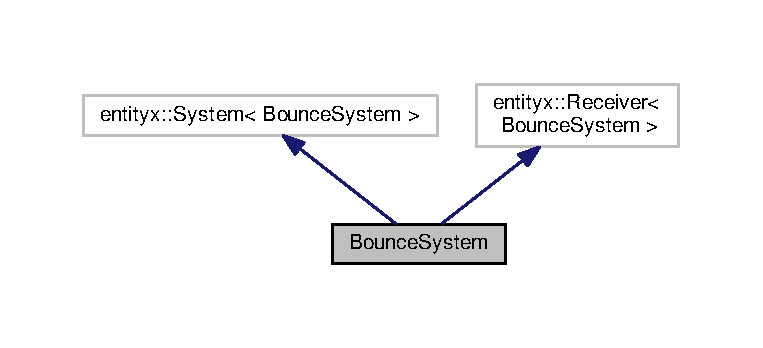
\includegraphics[width=350pt]{classBounceSystem__inherit__graph}
\end{center}
\end{figure}


Collaboration diagram for Bounce\+System\+:
\nopagebreak
\begin{figure}[H]
\begin{center}
\leavevmode
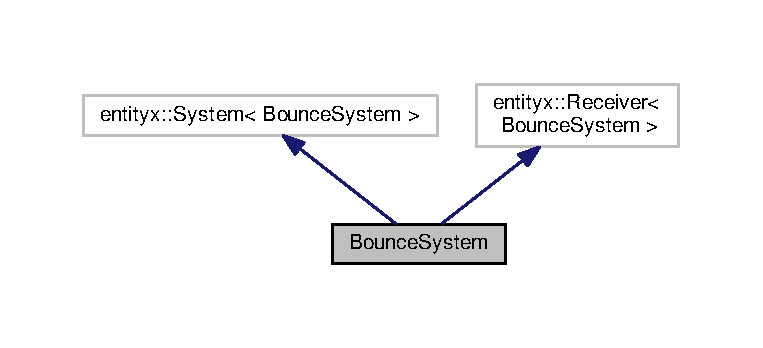
\includegraphics[width=350pt]{classBounceSystem__coll__graph}
\end{center}
\end{figure}
\subsection*{Public Member Functions}
\begin{DoxyCompactItemize}
\item 
\hyperlink{classBounceSystem_aefde06fe082b4ae32d34022b291a47e1}{Bounce\+System} (sf\+::\+Render\+Target \&target)
\item 
void \hyperlink{classBounceSystem_a64c3ae9db2a670af61b47be39c4fb353}{configure} (ex\+::\+Event\+Manager \&events) override
\item 
void \hyperlink{classBounceSystem_aeae5238af04e5eec67acd6ad897b9c3f}{update} (ex\+::\+Entity\+Manager \&es, ex\+::\+Event\+Manager \&events, ex\+::\+Time\+Delta dt) override
\item 
void \hyperlink{classBounceSystem_a26bcb419f819afb3c4a19364585c72a3}{receive} (const \hyperlink{structCollisionEvent}{Collision\+Event} \&coll\+\_\+event)
\end{DoxyCompactItemize}
\subsection*{Static Public Member Functions}
\begin{DoxyCompactItemize}
\item 
static void \hyperlink{classBounceSystem_ae7fdd15d7e5dffed1ec3fa997cc64e8f}{reverse} (float \&value)
\end{DoxyCompactItemize}


\subsection{Constructor \& Destructor Documentation}
\mbox{\Hypertarget{classBounceSystem_aefde06fe082b4ae32d34022b291a47e1}\label{classBounceSystem_aefde06fe082b4ae32d34022b291a47e1}} 
\index{Bounce\+System@{Bounce\+System}!Bounce\+System@{Bounce\+System}}
\index{Bounce\+System@{Bounce\+System}!Bounce\+System@{Bounce\+System}}
\subsubsection{\texorpdfstring{Bounce\+System()}{BounceSystem()}}
{\footnotesize\ttfamily Bounce\+System\+::\+Bounce\+System (\begin{DoxyParamCaption}\item[{sf\+::\+Render\+Target \&}]{target }\end{DoxyParamCaption})\hspace{0.3cm}{\ttfamily [inline]}, {\ttfamily [explicit]}}



\subsection{Member Function Documentation}
\mbox{\Hypertarget{classBounceSystem_a64c3ae9db2a670af61b47be39c4fb353}\label{classBounceSystem_a64c3ae9db2a670af61b47be39c4fb353}} 
\index{Bounce\+System@{Bounce\+System}!configure@{configure}}
\index{configure@{configure}!Bounce\+System@{Bounce\+System}}
\subsubsection{\texorpdfstring{configure()}{configure()}}
{\footnotesize\ttfamily void Bounce\+System\+::configure (\begin{DoxyParamCaption}\item[{ex\+::\+Event\+Manager \&}]{events }\end{DoxyParamCaption})\hspace{0.3cm}{\ttfamily [override]}}

\mbox{\Hypertarget{classBounceSystem_a26bcb419f819afb3c4a19364585c72a3}\label{classBounceSystem_a26bcb419f819afb3c4a19364585c72a3}} 
\index{Bounce\+System@{Bounce\+System}!receive@{receive}}
\index{receive@{receive}!Bounce\+System@{Bounce\+System}}
\subsubsection{\texorpdfstring{receive()}{receive()}}
{\footnotesize\ttfamily void Bounce\+System\+::receive (\begin{DoxyParamCaption}\item[{const \hyperlink{structCollisionEvent}{Collision\+Event} \&}]{coll\+\_\+event }\end{DoxyParamCaption})}

\mbox{\Hypertarget{classBounceSystem_ae7fdd15d7e5dffed1ec3fa997cc64e8f}\label{classBounceSystem_ae7fdd15d7e5dffed1ec3fa997cc64e8f}} 
\index{Bounce\+System@{Bounce\+System}!reverse@{reverse}}
\index{reverse@{reverse}!Bounce\+System@{Bounce\+System}}
\subsubsection{\texorpdfstring{reverse()}{reverse()}}
{\footnotesize\ttfamily void Bounce\+System\+::reverse (\begin{DoxyParamCaption}\item[{float \&}]{value }\end{DoxyParamCaption})\hspace{0.3cm}{\ttfamily [static]}}

\mbox{\Hypertarget{classBounceSystem_aeae5238af04e5eec67acd6ad897b9c3f}\label{classBounceSystem_aeae5238af04e5eec67acd6ad897b9c3f}} 
\index{Bounce\+System@{Bounce\+System}!update@{update}}
\index{update@{update}!Bounce\+System@{Bounce\+System}}
\subsubsection{\texorpdfstring{update()}{update()}}
{\footnotesize\ttfamily void Bounce\+System\+::update (\begin{DoxyParamCaption}\item[{ex\+::\+Entity\+Manager \&}]{es,  }\item[{ex\+::\+Event\+Manager \&}]{events,  }\item[{ex\+::\+Time\+Delta}]{dt }\end{DoxyParamCaption})\hspace{0.3cm}{\ttfamily [override]}}



The documentation for this class was generated from the following files\+:\begin{DoxyCompactItemize}
\item 
deprecated/\hyperlink{bounce__system_8h}{bounce\+\_\+system.\+h}\item 
deprecated/\hyperlink{bounce__system_8cpp}{bounce\+\_\+system.\+cpp}\end{DoxyCompactItemize}

\hypertarget{structCircleShape}{}\section{Circle\+Shape Struct Reference}
\label{structCircleShape}\index{Circle\+Shape@{Circle\+Shape}}


{\ttfamily \#include $<$shapes.\+h$>$}

\subsection*{Public Member Functions}
\begin{DoxyCompactItemize}
\item 
\hyperlink{structCircleShape_a548a4dbaae0d3fb2e4e3c6a0eb61297b}{Circle\+Shape} (float \hyperlink{structCircleShape_a4f50a8ecffa8f194062a71d584338a4a}{radius})
\end{DoxyCompactItemize}
\subsection*{Public Attributes}
\begin{DoxyCompactItemize}
\item 
float \hyperlink{structCircleShape_a4f50a8ecffa8f194062a71d584338a4a}{radius}
\end{DoxyCompactItemize}


\subsection{Constructor \& Destructor Documentation}
\mbox{\Hypertarget{structCircleShape_a548a4dbaae0d3fb2e4e3c6a0eb61297b}\label{structCircleShape_a548a4dbaae0d3fb2e4e3c6a0eb61297b}} 
\index{Circle\+Shape@{Circle\+Shape}!Circle\+Shape@{Circle\+Shape}}
\index{Circle\+Shape@{Circle\+Shape}!Circle\+Shape@{Circle\+Shape}}
\subsubsection{\texorpdfstring{Circle\+Shape()}{CircleShape()}}
{\footnotesize\ttfamily Circle\+Shape\+::\+Circle\+Shape (\begin{DoxyParamCaption}\item[{float}]{radius }\end{DoxyParamCaption})\hspace{0.3cm}{\ttfamily [inline]}}



\subsection{Member Data Documentation}
\mbox{\Hypertarget{structCircleShape_a4f50a8ecffa8f194062a71d584338a4a}\label{structCircleShape_a4f50a8ecffa8f194062a71d584338a4a}} 
\index{Circle\+Shape@{Circle\+Shape}!radius@{radius}}
\index{radius@{radius}!Circle\+Shape@{Circle\+Shape}}
\subsubsection{\texorpdfstring{radius}{radius}}
{\footnotesize\ttfamily float Circle\+Shape\+::radius}



The documentation for this struct was generated from the following file\+:\begin{DoxyCompactItemize}
\item 
components/\hyperlink{shapes_8h}{shapes.\+h}\end{DoxyCompactItemize}

\hypertarget{structCollideable}{}\section{Collideable Struct Reference}
\label{structCollideable}\index{Collideable@{Collideable}}


{\ttfamily \#include $<$collideable.\+h$>$}



The documentation for this struct was generated from the following file\+:\begin{DoxyCompactItemize}
\item 
components/\hyperlink{collideable_8h}{collideable.\+h}\end{DoxyCompactItemize}

\hypertarget{structCollisionEvent}{}\section{Collision\+Event Struct Reference}
\label{structCollisionEvent}\index{Collision\+Event@{Collision\+Event}}


{\ttfamily \#include $<$collision\+\_\+event.\+h$>$}

\subsection*{Public Member Functions}
\begin{DoxyCompactItemize}
\item 
\hyperlink{structCollisionEvent_a09fc3a9da18648340e9442cfb511c34c}{Collision\+Event} (ex\+::\+Entity \hyperlink{structCollisionEvent_ab04ed3aa79522e3f296245e39f7ba846}{left}, entityx\+::\+Entity \hyperlink{structCollisionEvent_a665ecc7b6b9b4d54b44ab9d0d9930984}{right})
\end{DoxyCompactItemize}
\subsection*{Public Attributes}
\begin{DoxyCompactItemize}
\item 
entityx\+::\+Entity \hyperlink{structCollisionEvent_ab04ed3aa79522e3f296245e39f7ba846}{left}
\item 
entityx\+::\+Entity \hyperlink{structCollisionEvent_a665ecc7b6b9b4d54b44ab9d0d9930984}{right}
\end{DoxyCompactItemize}


\subsection{Constructor \& Destructor Documentation}
\mbox{\Hypertarget{structCollisionEvent_a09fc3a9da18648340e9442cfb511c34c}\label{structCollisionEvent_a09fc3a9da18648340e9442cfb511c34c}} 
\index{Collision\+Event@{Collision\+Event}!Collision\+Event@{Collision\+Event}}
\index{Collision\+Event@{Collision\+Event}!Collision\+Event@{Collision\+Event}}
\subsubsection{\texorpdfstring{Collision\+Event()}{CollisionEvent()}}
{\footnotesize\ttfamily Collision\+Event\+::\+Collision\+Event (\begin{DoxyParamCaption}\item[{ex\+::\+Entity}]{left,  }\item[{entityx\+::\+Entity}]{right }\end{DoxyParamCaption})\hspace{0.3cm}{\ttfamily [inline]}}



\subsection{Member Data Documentation}
\mbox{\Hypertarget{structCollisionEvent_ab04ed3aa79522e3f296245e39f7ba846}\label{structCollisionEvent_ab04ed3aa79522e3f296245e39f7ba846}} 
\index{Collision\+Event@{Collision\+Event}!left@{left}}
\index{left@{left}!Collision\+Event@{Collision\+Event}}
\subsubsection{\texorpdfstring{left}{left}}
{\footnotesize\ttfamily entityx\+::\+Entity Collision\+Event\+::left}

\mbox{\Hypertarget{structCollisionEvent_a665ecc7b6b9b4d54b44ab9d0d9930984}\label{structCollisionEvent_a665ecc7b6b9b4d54b44ab9d0d9930984}} 
\index{Collision\+Event@{Collision\+Event}!right@{right}}
\index{right@{right}!Collision\+Event@{Collision\+Event}}
\subsubsection{\texorpdfstring{right}{right}}
{\footnotesize\ttfamily entityx\+::\+Entity Collision\+Event\+::right}



The documentation for this struct was generated from the following file\+:\begin{DoxyCompactItemize}
\item 
events/\hyperlink{collision__event_8h}{collision\+\_\+event.\+h}\end{DoxyCompactItemize}

\hypertarget{classCollisionSystem}{}\section{Collision\+System Class Reference}
\label{classCollisionSystem}\index{Collision\+System@{Collision\+System}}


{\ttfamily \#include $<$collision\+\_\+system.\+h$>$}



Inheritance diagram for Collision\+System\+:
\nopagebreak
\begin{figure}[H]
\begin{center}
\leavevmode
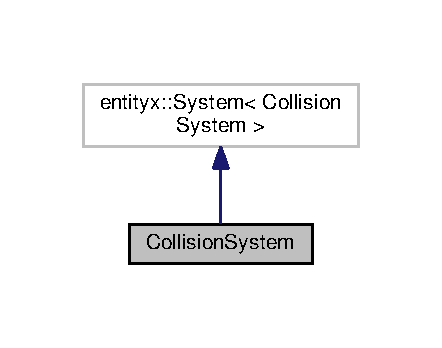
\includegraphics[width=212pt]{classCollisionSystem__inherit__graph}
\end{center}
\end{figure}


Collaboration diagram for Collision\+System\+:
\nopagebreak
\begin{figure}[H]
\begin{center}
\leavevmode
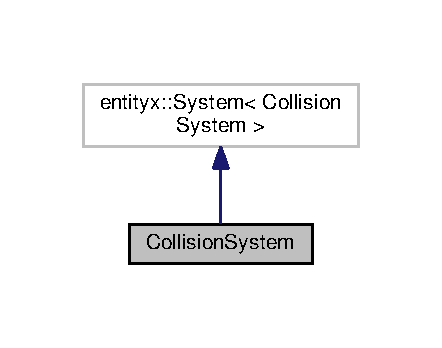
\includegraphics[width=212pt]{classCollisionSystem__coll__graph}
\end{center}
\end{figure}
\subsection*{Public Member Functions}
\begin{DoxyCompactItemize}
\item 
\hyperlink{classCollisionSystem_a3d6fbd73a8e9e123413d8907bc4a64a6}{Collision\+System} (sf\+::\+Render\+Target \&target)
\item 
void \hyperlink{classCollisionSystem_a1206810c1190c25db4a27f70d0e8d27d}{update} (entityx\+::\+Entity\+Manager \&es, entityx\+::\+Event\+Manager \&events, entityx\+::\+Time\+Delta dt) override
\end{DoxyCompactItemize}


\subsection{Constructor \& Destructor Documentation}
\mbox{\Hypertarget{classCollisionSystem_a3d6fbd73a8e9e123413d8907bc4a64a6}\label{classCollisionSystem_a3d6fbd73a8e9e123413d8907bc4a64a6}} 
\index{Collision\+System@{Collision\+System}!Collision\+System@{Collision\+System}}
\index{Collision\+System@{Collision\+System}!Collision\+System@{Collision\+System}}
\subsubsection{\texorpdfstring{Collision\+System()}{CollisionSystem()}}
{\footnotesize\ttfamily Collision\+System\+::\+Collision\+System (\begin{DoxyParamCaption}\item[{sf\+::\+Render\+Target \&}]{target }\end{DoxyParamCaption})\hspace{0.3cm}{\ttfamily [explicit]}}



\subsection{Member Function Documentation}
\mbox{\Hypertarget{classCollisionSystem_a1206810c1190c25db4a27f70d0e8d27d}\label{classCollisionSystem_a1206810c1190c25db4a27f70d0e8d27d}} 
\index{Collision\+System@{Collision\+System}!update@{update}}
\index{update@{update}!Collision\+System@{Collision\+System}}
\subsubsection{\texorpdfstring{update()}{update()}}
{\footnotesize\ttfamily void Collision\+System\+::update (\begin{DoxyParamCaption}\item[{entityx\+::\+Entity\+Manager \&}]{es,  }\item[{entityx\+::\+Event\+Manager \&}]{events,  }\item[{entityx\+::\+Time\+Delta}]{dt }\end{DoxyParamCaption})\hspace{0.3cm}{\ttfamily [override]}}



The documentation for this class was generated from the following files\+:\begin{DoxyCompactItemize}
\item 
deprecated/\hyperlink{collision__system_8h}{collision\+\_\+system.\+h}\item 
deprecated/\hyperlink{collision__system_8cpp}{collision\+\_\+system.\+cpp}\end{DoxyCompactItemize}

\hypertarget{classEcsManager}{}\section{Ecs\+Manager Class Reference}
\label{classEcsManager}\index{Ecs\+Manager@{Ecs\+Manager}}


Inheritance diagram for Ecs\+Manager\+:\nopagebreak
\begin{figure}[H]
\begin{center}
\leavevmode
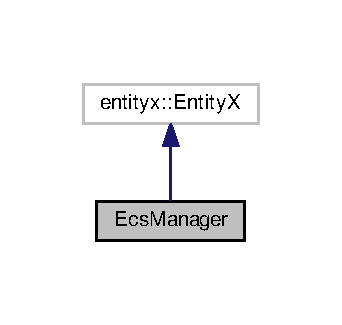
\includegraphics[width=164pt]{classEcsManager__inherit__graph}
\end{center}
\end{figure}


Collaboration diagram for Ecs\+Manager\+:\nopagebreak
\begin{figure}[H]
\begin{center}
\leavevmode
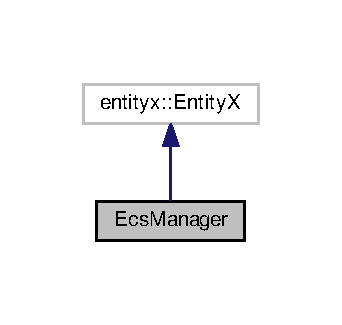
\includegraphics[width=164pt]{classEcsManager__coll__graph}
\end{center}
\end{figure}
\subsection*{Public Member Functions}
\begin{DoxyCompactItemize}
\item 
\hyperlink{classEcsManager_aa34cfb8983951b281bcfc59e9625f9a0}{Ecs\+Manager} (sf\+::\+Render\+Target \&target, sf\+::\+Font \&font)
\item 
void \hyperlink{classEcsManager_a28fa50f9ab6b01f06dd9cfb6f7d7a1b7}{update} (ex\+::\+Time\+Delta dt)
\end{DoxyCompactItemize}


\subsection{Constructor \& Destructor Documentation}
\mbox{\Hypertarget{classEcsManager_aa34cfb8983951b281bcfc59e9625f9a0}\label{classEcsManager_aa34cfb8983951b281bcfc59e9625f9a0}} 
\index{Ecs\+Manager@{Ecs\+Manager}!Ecs\+Manager@{Ecs\+Manager}}
\index{Ecs\+Manager@{Ecs\+Manager}!Ecs\+Manager@{Ecs\+Manager}}
\subsubsection{\texorpdfstring{Ecs\+Manager()}{EcsManager()}}
{\footnotesize\ttfamily Ecs\+Manager\+::\+Ecs\+Manager (\begin{DoxyParamCaption}\item[{sf\+::\+Render\+Target \&}]{target,  }\item[{sf\+::\+Font \&}]{font }\end{DoxyParamCaption})\hspace{0.3cm}{\ttfamily [inline]}, {\ttfamily [explicit]}}



\subsection{Member Function Documentation}
\mbox{\Hypertarget{classEcsManager_a28fa50f9ab6b01f06dd9cfb6f7d7a1b7}\label{classEcsManager_a28fa50f9ab6b01f06dd9cfb6f7d7a1b7}} 
\index{Ecs\+Manager@{Ecs\+Manager}!update@{update}}
\index{update@{update}!Ecs\+Manager@{Ecs\+Manager}}
\subsubsection{\texorpdfstring{update()}{update()}}
{\footnotesize\ttfamily void Ecs\+Manager\+::update (\begin{DoxyParamCaption}\item[{ex\+::\+Time\+Delta}]{dt }\end{DoxyParamCaption})\hspace{0.3cm}{\ttfamily [inline]}}



The documentation for this class was generated from the following file\+:\begin{DoxyCompactItemize}
\item 
\hyperlink{main_8cpp}{main.\+cpp}\end{DoxyCompactItemize}

\hypertarget{classEntitySpawnedEvent}{}\section{Entity\+Spawned\+Event Class Reference}
\label{classEntitySpawnedEvent}\index{Entity\+Spawned\+Event@{Entity\+Spawned\+Event}}


{\ttfamily \#include $<$Entity\+Spawned\+Event.\+h$>$}

\subsection*{Public Member Functions}
\begin{DoxyCompactItemize}
\item 
\hyperlink{classEntitySpawnedEvent_ad5622458ef3448dec870b2f68d009a3d}{Entity\+Spawned\+Event} (entityx\+::\+Entity \hyperlink{classEntitySpawnedEvent_a5c5e65c69bfd2783367202115bcced3c}{entity})
\end{DoxyCompactItemize}
\subsection*{Public Attributes}
\begin{DoxyCompactItemize}
\item 
entityx\+::\+Entity \hyperlink{classEntitySpawnedEvent_a5c5e65c69bfd2783367202115bcced3c}{entity}
\end{DoxyCompactItemize}


\subsection{Constructor \& Destructor Documentation}
\mbox{\Hypertarget{classEntitySpawnedEvent_ad5622458ef3448dec870b2f68d009a3d}\label{classEntitySpawnedEvent_ad5622458ef3448dec870b2f68d009a3d}} 
\index{Entity\+Spawned\+Event@{Entity\+Spawned\+Event}!Entity\+Spawned\+Event@{Entity\+Spawned\+Event}}
\index{Entity\+Spawned\+Event@{Entity\+Spawned\+Event}!Entity\+Spawned\+Event@{Entity\+Spawned\+Event}}
\subsubsection{\texorpdfstring{Entity\+Spawned\+Event()}{EntitySpawnedEvent()}}
{\footnotesize\ttfamily Entity\+Spawned\+Event\+::\+Entity\+Spawned\+Event (\begin{DoxyParamCaption}\item[{entityx\+::\+Entity}]{entity }\end{DoxyParamCaption})\hspace{0.3cm}{\ttfamily [inline]}}



\subsection{Member Data Documentation}
\mbox{\Hypertarget{classEntitySpawnedEvent_a5c5e65c69bfd2783367202115bcced3c}\label{classEntitySpawnedEvent_a5c5e65c69bfd2783367202115bcced3c}} 
\index{Entity\+Spawned\+Event@{Entity\+Spawned\+Event}!entity@{entity}}
\index{entity@{entity}!Entity\+Spawned\+Event@{Entity\+Spawned\+Event}}
\subsubsection{\texorpdfstring{entity}{entity}}
{\footnotesize\ttfamily entityx\+::\+Entity Entity\+Spawned\+Event\+::entity}



The documentation for this class was generated from the following file\+:\begin{DoxyCompactItemize}
\item 
events/\hyperlink{EntitySpawnedEvent_8h}{Entity\+Spawned\+Event.\+h}\end{DoxyCompactItemize}

\hypertarget{classFpsCounter}{}\section{Fps\+Counter Class Reference}
\label{classFpsCounter}\index{Fps\+Counter@{Fps\+Counter}}


{\ttfamily \#include $<$util.\+h$>$}

\subsection*{Public Member Functions}
\begin{DoxyCompactItemize}
\item 
float \hyperlink{classFpsCounter_ae9957d6f9e8d1d0710ca73eca43f7e5b}{update} (float timepassed)
\end{DoxyCompactItemize}


\subsection{Member Function Documentation}
\mbox{\Hypertarget{classFpsCounter_ae9957d6f9e8d1d0710ca73eca43f7e5b}\label{classFpsCounter_ae9957d6f9e8d1d0710ca73eca43f7e5b}} 
\index{Fps\+Counter@{Fps\+Counter}!update@{update}}
\index{update@{update}!Fps\+Counter@{Fps\+Counter}}
\subsubsection{\texorpdfstring{update()}{update()}}
{\footnotesize\ttfamily float Fps\+Counter\+::update (\begin{DoxyParamCaption}\item[{float}]{timepassed }\end{DoxyParamCaption})}



The documentation for this class was generated from the following files\+:\begin{DoxyCompactItemize}
\item 
\hyperlink{util_8h}{util.\+h}\item 
\hyperlink{util_8cpp}{util.\+cpp}\end{DoxyCompactItemize}

\hypertarget{classGravitySystem}{}\section{Gravity\+System Class Reference}
\label{classGravitySystem}\index{Gravity\+System@{Gravity\+System}}


{\ttfamily \#include $<$gravity\+\_\+system.\+h$>$}



Inheritance diagram for Gravity\+System\+:
\nopagebreak
\begin{figure}[H]
\begin{center}
\leavevmode
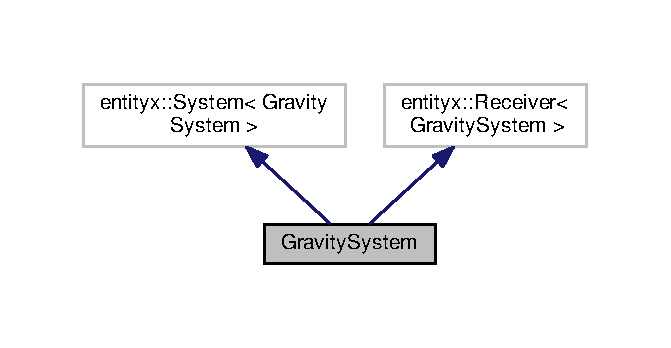
\includegraphics[width=322pt]{classGravitySystem__inherit__graph}
\end{center}
\end{figure}


Collaboration diagram for Gravity\+System\+:
\nopagebreak
\begin{figure}[H]
\begin{center}
\leavevmode
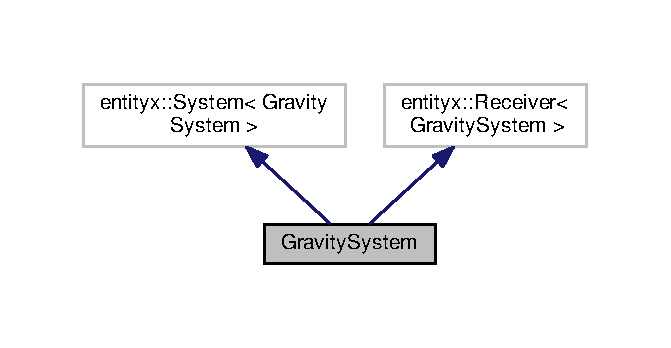
\includegraphics[width=322pt]{classGravitySystem__coll__graph}
\end{center}
\end{figure}
\subsection*{Public Member Functions}
\begin{DoxyCompactItemize}
\item 
\hyperlink{classGravitySystem_adf52a6e69ad42c81ebfe551093897bfc}{Gravity\+System} ()
\item 
void \hyperlink{classGravitySystem_a96d2addda17d0405ec82a1c6beb57b7a}{update} (ex\+::\+Entity\+Manager \&es, ex\+::\+Event\+Manager \&events, ex\+::\+Time\+Delta dt)
\item 
void \hyperlink{classGravitySystem_af53475dc43da2c55b71875ddb1f6bda5}{configure} (ex\+::\+Event\+Manager \&events) override
\item 
void \hyperlink{classGravitySystem_a9ccb1aae9dfbcbdd6c12a286010deddd}{receive} (const \hyperlink{classEntitySpawnedEvent}{Entity\+Spawned\+Event} \&entity\+\_\+spawned\+\_\+event)
\end{DoxyCompactItemize}


\subsection{Constructor \& Destructor Documentation}
\mbox{\Hypertarget{classGravitySystem_adf52a6e69ad42c81ebfe551093897bfc}\label{classGravitySystem_adf52a6e69ad42c81ebfe551093897bfc}} 
\index{Gravity\+System@{Gravity\+System}!Gravity\+System@{Gravity\+System}}
\index{Gravity\+System@{Gravity\+System}!Gravity\+System@{Gravity\+System}}
\subsubsection{\texorpdfstring{Gravity\+System()}{GravitySystem()}}
{\footnotesize\ttfamily Gravity\+System\+::\+Gravity\+System (\begin{DoxyParamCaption}{ }\end{DoxyParamCaption})\hspace{0.3cm}{\ttfamily [inline]}, {\ttfamily [explicit]}}



\subsection{Member Function Documentation}
\mbox{\Hypertarget{classGravitySystem_af53475dc43da2c55b71875ddb1f6bda5}\label{classGravitySystem_af53475dc43da2c55b71875ddb1f6bda5}} 
\index{Gravity\+System@{Gravity\+System}!configure@{configure}}
\index{configure@{configure}!Gravity\+System@{Gravity\+System}}
\subsubsection{\texorpdfstring{configure()}{configure()}}
{\footnotesize\ttfamily void Gravity\+System\+::configure (\begin{DoxyParamCaption}\item[{ex\+::\+Event\+Manager \&}]{events }\end{DoxyParamCaption})\hspace{0.3cm}{\ttfamily [inline]}, {\ttfamily [override]}}

\mbox{\Hypertarget{classGravitySystem_a9ccb1aae9dfbcbdd6c12a286010deddd}\label{classGravitySystem_a9ccb1aae9dfbcbdd6c12a286010deddd}} 
\index{Gravity\+System@{Gravity\+System}!receive@{receive}}
\index{receive@{receive}!Gravity\+System@{Gravity\+System}}
\subsubsection{\texorpdfstring{receive()}{receive()}}
{\footnotesize\ttfamily void Gravity\+System\+::receive (\begin{DoxyParamCaption}\item[{const \hyperlink{classEntitySpawnedEvent}{Entity\+Spawned\+Event} \&}]{entity\+\_\+spawned\+\_\+event }\end{DoxyParamCaption})\hspace{0.3cm}{\ttfamily [inline]}}

\mbox{\Hypertarget{classGravitySystem_a96d2addda17d0405ec82a1c6beb57b7a}\label{classGravitySystem_a96d2addda17d0405ec82a1c6beb57b7a}} 
\index{Gravity\+System@{Gravity\+System}!update@{update}}
\index{update@{update}!Gravity\+System@{Gravity\+System}}
\subsubsection{\texorpdfstring{update()}{update()}}
{\footnotesize\ttfamily void Gravity\+System\+::update (\begin{DoxyParamCaption}\item[{ex\+::\+Entity\+Manager \&}]{es,  }\item[{ex\+::\+Event\+Manager \&}]{events,  }\item[{ex\+::\+Time\+Delta}]{dt }\end{DoxyParamCaption})\hspace{0.3cm}{\ttfamily [inline]}}



The documentation for this class was generated from the following file\+:\begin{DoxyCompactItemize}
\item 
systems/\hyperlink{gravity__system_8h}{gravity\+\_\+system.\+h}\end{DoxyCompactItemize}

\hypertarget{classInfoDrawSystem}{}\section{Info\+Draw\+System Class Reference}
\label{classInfoDrawSystem}\index{Info\+Draw\+System@{Info\+Draw\+System}}


{\ttfamily \#include $<$info\+\_\+draw\+\_\+system.\+h$>$}



Inheritance diagram for Info\+Draw\+System\+:
\nopagebreak
\begin{figure}[H]
\begin{center}
\leavevmode
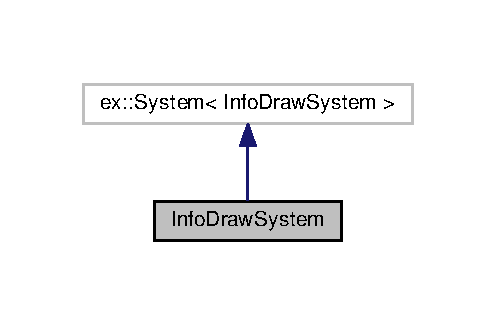
\includegraphics[width=238pt]{classInfoDrawSystem__inherit__graph}
\end{center}
\end{figure}


Collaboration diagram for Info\+Draw\+System\+:
\nopagebreak
\begin{figure}[H]
\begin{center}
\leavevmode
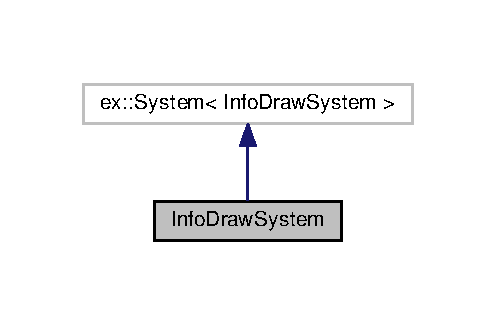
\includegraphics[width=238pt]{classInfoDrawSystem__coll__graph}
\end{center}
\end{figure}
\subsection*{Public Member Functions}
\begin{DoxyCompactItemize}
\item 
\hyperlink{classInfoDrawSystem_a6ddca785e40f494d5973a8b957a76873}{Info\+Draw\+System} (sf\+::\+Render\+Target \&target, sf\+::\+Font \&font)
\item 
void \hyperlink{classInfoDrawSystem_aac0a0e5f1595857ca8ab47c17ea3e62e}{update} (ex\+::\+Entity\+Manager \&entities, ex\+::\+Event\+Manager \&events, ex\+::\+Time\+Delta dt) override
\end{DoxyCompactItemize}


\subsection{Constructor \& Destructor Documentation}
\mbox{\Hypertarget{classInfoDrawSystem_a6ddca785e40f494d5973a8b957a76873}\label{classInfoDrawSystem_a6ddca785e40f494d5973a8b957a76873}} 
\index{Info\+Draw\+System@{Info\+Draw\+System}!Info\+Draw\+System@{Info\+Draw\+System}}
\index{Info\+Draw\+System@{Info\+Draw\+System}!Info\+Draw\+System@{Info\+Draw\+System}}
\subsubsection{\texorpdfstring{Info\+Draw\+System()}{InfoDrawSystem()}}
{\footnotesize\ttfamily Info\+Draw\+System\+::\+Info\+Draw\+System (\begin{DoxyParamCaption}\item[{sf\+::\+Render\+Target \&}]{target,  }\item[{sf\+::\+Font \&}]{font }\end{DoxyParamCaption})\hspace{0.3cm}{\ttfamily [explicit]}}



\subsection{Member Function Documentation}
\mbox{\Hypertarget{classInfoDrawSystem_aac0a0e5f1595857ca8ab47c17ea3e62e}\label{classInfoDrawSystem_aac0a0e5f1595857ca8ab47c17ea3e62e}} 
\index{Info\+Draw\+System@{Info\+Draw\+System}!update@{update}}
\index{update@{update}!Info\+Draw\+System@{Info\+Draw\+System}}
\subsubsection{\texorpdfstring{update()}{update()}}
{\footnotesize\ttfamily void Info\+Draw\+System\+::update (\begin{DoxyParamCaption}\item[{ex\+::\+Entity\+Manager \&}]{entities,  }\item[{ex\+::\+Event\+Manager \&}]{events,  }\item[{ex\+::\+Time\+Delta}]{dt }\end{DoxyParamCaption})\hspace{0.3cm}{\ttfamily [override]}}



The documentation for this class was generated from the following files\+:\begin{DoxyCompactItemize}
\item 
systems/\hyperlink{info__draw__system_8h}{info\+\_\+draw\+\_\+system.\+h}\item 
systems/\hyperlink{info__draw__system_8cpp}{info\+\_\+draw\+\_\+system.\+cpp}\end{DoxyCompactItemize}

\hypertarget{classMass}{}\section{Mass Class Reference}
\label{classMass}\index{Mass@{Mass}}


{\ttfamily \#include $<$mass.\+h$>$}

\subsection*{Public Member Functions}
\begin{DoxyCompactItemize}
\item 
\hyperlink{classMass_ae7d9a813ae791bc44fbe52e18eef223e}{Mass} (float \hyperlink{classMass_a1c332d2b4b785512fc6fb77f2cf3f805}{value})
\end{DoxyCompactItemize}
\subsection*{Public Attributes}
\begin{DoxyCompactItemize}
\item 
float \hyperlink{classMass_a1c332d2b4b785512fc6fb77f2cf3f805}{value}
\end{DoxyCompactItemize}


\subsection{Constructor \& Destructor Documentation}
\mbox{\Hypertarget{classMass_ae7d9a813ae791bc44fbe52e18eef223e}\label{classMass_ae7d9a813ae791bc44fbe52e18eef223e}} 
\index{Mass@{Mass}!Mass@{Mass}}
\index{Mass@{Mass}!Mass@{Mass}}
\subsubsection{\texorpdfstring{Mass()}{Mass()}}
{\footnotesize\ttfamily Mass\+::\+Mass (\begin{DoxyParamCaption}\item[{float}]{value }\end{DoxyParamCaption})\hspace{0.3cm}{\ttfamily [inline]}}



\subsection{Member Data Documentation}
\mbox{\Hypertarget{classMass_a1c332d2b4b785512fc6fb77f2cf3f805}\label{classMass_a1c332d2b4b785512fc6fb77f2cf3f805}} 
\index{Mass@{Mass}!value@{value}}
\index{value@{value}!Mass@{Mass}}
\subsubsection{\texorpdfstring{value}{value}}
{\footnotesize\ttfamily float Mass\+::value}



The documentation for this class was generated from the following file\+:\begin{DoxyCompactItemize}
\item 
components/\hyperlink{mass_8h}{mass.\+h}\end{DoxyCompactItemize}

\hypertarget{structOpacitySystem}{}\section{Opacity\+System Struct Reference}
\label{structOpacitySystem}\index{Opacity\+System@{Opacity\+System}}


{\ttfamily \#include $<$opacity\+\_\+system.\+h$>$}



Inheritance diagram for Opacity\+System\+:
\nopagebreak
\begin{figure}[H]
\begin{center}
\leavevmode
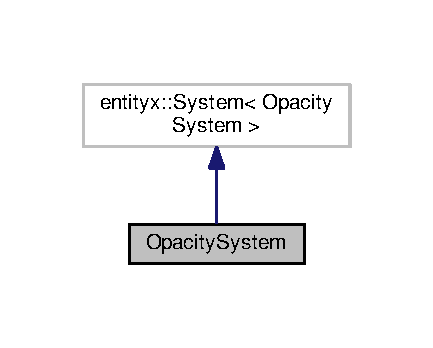
\includegraphics[width=208pt]{structOpacitySystem__inherit__graph}
\end{center}
\end{figure}


Collaboration diagram for Opacity\+System\+:
\nopagebreak
\begin{figure}[H]
\begin{center}
\leavevmode
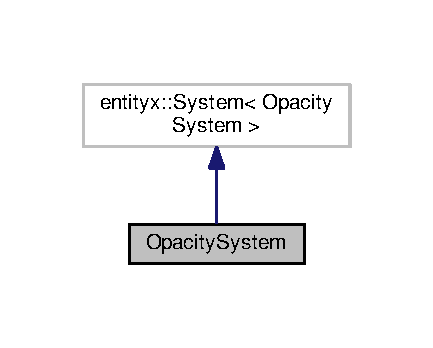
\includegraphics[width=208pt]{structOpacitySystem__coll__graph}
\end{center}
\end{figure}
\subsection*{Public Member Functions}
\begin{DoxyCompactItemize}
\item 
void \hyperlink{structOpacitySystem_afaf8a988027dcfe4320c119837d10515}{update} (entityx\+::\+Entity\+Manager \&es, entityx\+::\+Event\+Manager \&events, entityx\+::\+Time\+Delta dt) override
\end{DoxyCompactItemize}


\subsection{Member Function Documentation}
\mbox{\Hypertarget{structOpacitySystem_afaf8a988027dcfe4320c119837d10515}\label{structOpacitySystem_afaf8a988027dcfe4320c119837d10515}} 
\index{Opacity\+System@{Opacity\+System}!update@{update}}
\index{update@{update}!Opacity\+System@{Opacity\+System}}
\subsubsection{\texorpdfstring{update()}{update()}}
{\footnotesize\ttfamily void Opacity\+System\+::update (\begin{DoxyParamCaption}\item[{entityx\+::\+Entity\+Manager \&}]{es,  }\item[{entityx\+::\+Event\+Manager \&}]{events,  }\item[{entityx\+::\+Time\+Delta}]{dt }\end{DoxyParamCaption})\hspace{0.3cm}{\ttfamily [override]}}



The documentation for this struct was generated from the following files\+:\begin{DoxyCompactItemize}
\item 
systems/\hyperlink{opacity__system_8h}{opacity\+\_\+system.\+h}\item 
systems/\hyperlink{opacity__system_8cpp}{opacity\+\_\+system.\+cpp}\end{DoxyCompactItemize}

\hypertarget{classPhysicsSystem}{}\section{Physics\+System Class Reference}
\label{classPhysicsSystem}\index{Physics\+System@{Physics\+System}}


{\ttfamily \#include $<$physics\+\_\+system.\+h$>$}



Inheritance diagram for Physics\+System\+:
\nopagebreak
\begin{figure}[H]
\begin{center}
\leavevmode
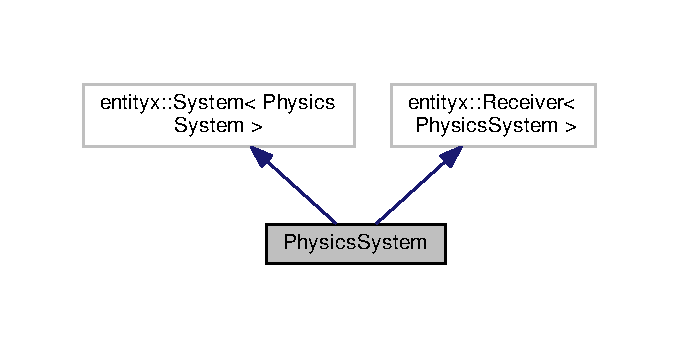
\includegraphics[width=326pt]{classPhysicsSystem__inherit__graph}
\end{center}
\end{figure}


Collaboration diagram for Physics\+System\+:
\nopagebreak
\begin{figure}[H]
\begin{center}
\leavevmode
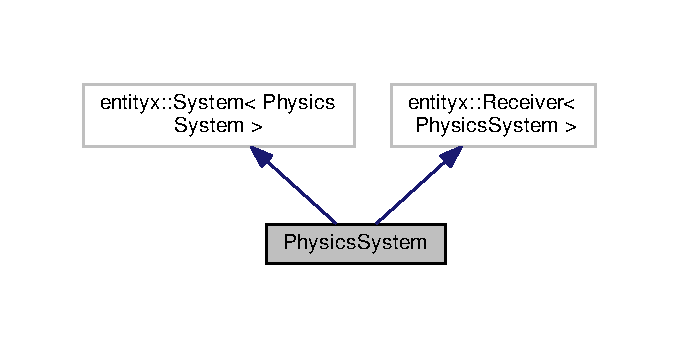
\includegraphics[width=326pt]{classPhysicsSystem__coll__graph}
\end{center}
\end{figure}
\subsection*{Public Member Functions}
\begin{DoxyCompactItemize}
\item 
\hyperlink{classPhysicsSystem_a4960fbd046fb332a5faa36fb5028e7c5}{Physics\+System} ()
\item 
void \hyperlink{classPhysicsSystem_a4e3674b18191bada7b4b79c5a4dcf5e2}{update} (ex\+::\+Entity\+Manager \&es, ex\+::\+Event\+Manager \&events, ex\+::\+Time\+Delta dt)
\item 
void \hyperlink{classPhysicsSystem_a8b42dc0a70e6da85e7dccad9897fd61c}{create\+Borders} (float width, float height)
\item 
void \hyperlink{classPhysicsSystem_ad5fb8504ea04b8a40146ddcb25f58861}{configure} (ex\+::\+Event\+Manager \&events) override
\item 
void \hyperlink{classPhysicsSystem_a41b6f92145e580bc80e903b13b6dfaa3}{receive} (const \hyperlink{classEntitySpawnedEvent}{Entity\+Spawned\+Event} \&entity\+\_\+spawned\+\_\+event)
\item 
void \hyperlink{classPhysicsSystem_ac7e8c1e5a616b42189de4605e4b6a687}{receive} (const ex\+::\+Entity\+Destroyed\+Event \&entity\+\_\+destroyed\+\_\+event)
\item 
void \hyperlink{classPhysicsSystem_a01fa32b7faab08192ae96e4520b8765a}{set\+Gravity} (float x, float y)
\end{DoxyCompactItemize}


\subsection{Constructor \& Destructor Documentation}
\mbox{\Hypertarget{classPhysicsSystem_a4960fbd046fb332a5faa36fb5028e7c5}\label{classPhysicsSystem_a4960fbd046fb332a5faa36fb5028e7c5}} 
\index{Physics\+System@{Physics\+System}!Physics\+System@{Physics\+System}}
\index{Physics\+System@{Physics\+System}!Physics\+System@{Physics\+System}}
\subsubsection{\texorpdfstring{Physics\+System()}{PhysicsSystem()}}
{\footnotesize\ttfamily Physics\+System\+::\+Physics\+System (\begin{DoxyParamCaption}{ }\end{DoxyParamCaption})\hspace{0.3cm}{\ttfamily [inline]}, {\ttfamily [explicit]}}



\subsection{Member Function Documentation}
\mbox{\Hypertarget{classPhysicsSystem_ad5fb8504ea04b8a40146ddcb25f58861}\label{classPhysicsSystem_ad5fb8504ea04b8a40146ddcb25f58861}} 
\index{Physics\+System@{Physics\+System}!configure@{configure}}
\index{configure@{configure}!Physics\+System@{Physics\+System}}
\subsubsection{\texorpdfstring{configure()}{configure()}}
{\footnotesize\ttfamily void Physics\+System\+::configure (\begin{DoxyParamCaption}\item[{ex\+::\+Event\+Manager \&}]{events }\end{DoxyParamCaption})\hspace{0.3cm}{\ttfamily [inline]}, {\ttfamily [override]}}

\mbox{\Hypertarget{classPhysicsSystem_a8b42dc0a70e6da85e7dccad9897fd61c}\label{classPhysicsSystem_a8b42dc0a70e6da85e7dccad9897fd61c}} 
\index{Physics\+System@{Physics\+System}!create\+Borders@{create\+Borders}}
\index{create\+Borders@{create\+Borders}!Physics\+System@{Physics\+System}}
\subsubsection{\texorpdfstring{create\+Borders()}{createBorders()}}
{\footnotesize\ttfamily void Physics\+System\+::create\+Borders (\begin{DoxyParamCaption}\item[{float}]{width,  }\item[{float}]{height }\end{DoxyParamCaption})\hspace{0.3cm}{\ttfamily [inline]}}

\mbox{\Hypertarget{classPhysicsSystem_a41b6f92145e580bc80e903b13b6dfaa3}\label{classPhysicsSystem_a41b6f92145e580bc80e903b13b6dfaa3}} 
\index{Physics\+System@{Physics\+System}!receive@{receive}}
\index{receive@{receive}!Physics\+System@{Physics\+System}}
\subsubsection{\texorpdfstring{receive()}{receive()}\hspace{0.1cm}{\footnotesize\ttfamily [1/2]}}
{\footnotesize\ttfamily void Physics\+System\+::receive (\begin{DoxyParamCaption}\item[{const \hyperlink{classEntitySpawnedEvent}{Entity\+Spawned\+Event} \&}]{entity\+\_\+spawned\+\_\+event }\end{DoxyParamCaption})\hspace{0.3cm}{\ttfamily [inline]}}

\mbox{\Hypertarget{classPhysicsSystem_ac7e8c1e5a616b42189de4605e4b6a687}\label{classPhysicsSystem_ac7e8c1e5a616b42189de4605e4b6a687}} 
\index{Physics\+System@{Physics\+System}!receive@{receive}}
\index{receive@{receive}!Physics\+System@{Physics\+System}}
\subsubsection{\texorpdfstring{receive()}{receive()}\hspace{0.1cm}{\footnotesize\ttfamily [2/2]}}
{\footnotesize\ttfamily void Physics\+System\+::receive (\begin{DoxyParamCaption}\item[{const ex\+::\+Entity\+Destroyed\+Event \&}]{entity\+\_\+destroyed\+\_\+event }\end{DoxyParamCaption})\hspace{0.3cm}{\ttfamily [inline]}}

\mbox{\Hypertarget{classPhysicsSystem_a01fa32b7faab08192ae96e4520b8765a}\label{classPhysicsSystem_a01fa32b7faab08192ae96e4520b8765a}} 
\index{Physics\+System@{Physics\+System}!set\+Gravity@{set\+Gravity}}
\index{set\+Gravity@{set\+Gravity}!Physics\+System@{Physics\+System}}
\subsubsection{\texorpdfstring{set\+Gravity()}{setGravity()}}
{\footnotesize\ttfamily void Physics\+System\+::set\+Gravity (\begin{DoxyParamCaption}\item[{float}]{x,  }\item[{float}]{y }\end{DoxyParamCaption})\hspace{0.3cm}{\ttfamily [inline]}}

\mbox{\Hypertarget{classPhysicsSystem_a4e3674b18191bada7b4b79c5a4dcf5e2}\label{classPhysicsSystem_a4e3674b18191bada7b4b79c5a4dcf5e2}} 
\index{Physics\+System@{Physics\+System}!update@{update}}
\index{update@{update}!Physics\+System@{Physics\+System}}
\subsubsection{\texorpdfstring{update()}{update()}}
{\footnotesize\ttfamily void Physics\+System\+::update (\begin{DoxyParamCaption}\item[{ex\+::\+Entity\+Manager \&}]{es,  }\item[{ex\+::\+Event\+Manager \&}]{events,  }\item[{ex\+::\+Time\+Delta}]{dt }\end{DoxyParamCaption})\hspace{0.3cm}{\ttfamily [inline]}}



The documentation for this class was generated from the following file\+:\begin{DoxyCompactItemize}
\item 
systems/\hyperlink{physics__system_8h}{physics\+\_\+system.\+h}\end{DoxyCompactItemize}

\hypertarget{classRandomMotionSystem}{}\section{Random\+Motion\+System Class Reference}
\label{classRandomMotionSystem}\index{Random\+Motion\+System@{Random\+Motion\+System}}


{\ttfamily \#include $<$random\+\_\+motion\+\_\+system.\+h$>$}



Inheritance diagram for Random\+Motion\+System\+:
\nopagebreak
\begin{figure}[H]
\begin{center}
\leavevmode
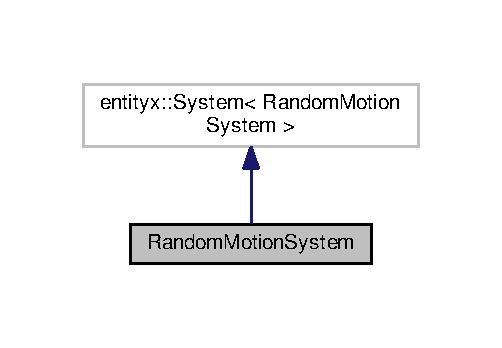
\includegraphics[width=241pt]{classRandomMotionSystem__inherit__graph}
\end{center}
\end{figure}


Collaboration diagram for Random\+Motion\+System\+:
\nopagebreak
\begin{figure}[H]
\begin{center}
\leavevmode
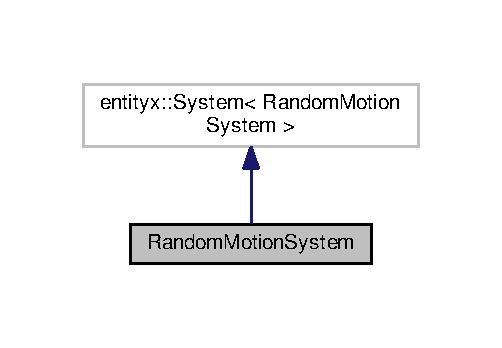
\includegraphics[width=241pt]{classRandomMotionSystem__coll__graph}
\end{center}
\end{figure}
\subsection*{Public Member Functions}
\begin{DoxyCompactItemize}
\item 
\hyperlink{classRandomMotionSystem_aef7a690b419355d36b52ec14d549fab2}{Random\+Motion\+System} ()
\item 
void \hyperlink{classRandomMotionSystem_af76eacfa2fbd4209ec02d77f8ef893d2}{update} (ex\+::\+Entity\+Manager \&es, ex\+::\+Event\+Manager \&events, ex\+::\+Time\+Delta dt) override
\item 
void \hyperlink{classRandomMotionSystem_a001b0eb8bce4321e0e3fbb14b3ba88a1}{accelerate\+Random} (\hyperlink{structBody}{Body} \&body)
\end{DoxyCompactItemize}


\subsection{Constructor \& Destructor Documentation}
\mbox{\Hypertarget{classRandomMotionSystem_aef7a690b419355d36b52ec14d549fab2}\label{classRandomMotionSystem_aef7a690b419355d36b52ec14d549fab2}} 
\index{Random\+Motion\+System@{Random\+Motion\+System}!Random\+Motion\+System@{Random\+Motion\+System}}
\index{Random\+Motion\+System@{Random\+Motion\+System}!Random\+Motion\+System@{Random\+Motion\+System}}
\subsubsection{\texorpdfstring{Random\+Motion\+System()}{RandomMotionSystem()}}
{\footnotesize\ttfamily Random\+Motion\+System\+::\+Random\+Motion\+System (\begin{DoxyParamCaption}{ }\end{DoxyParamCaption})\hspace{0.3cm}{\ttfamily [inline]}, {\ttfamily [explicit]}}



\subsection{Member Function Documentation}
\mbox{\Hypertarget{classRandomMotionSystem_a001b0eb8bce4321e0e3fbb14b3ba88a1}\label{classRandomMotionSystem_a001b0eb8bce4321e0e3fbb14b3ba88a1}} 
\index{Random\+Motion\+System@{Random\+Motion\+System}!accelerate\+Random@{accelerate\+Random}}
\index{accelerate\+Random@{accelerate\+Random}!Random\+Motion\+System@{Random\+Motion\+System}}
\subsubsection{\texorpdfstring{accelerate\+Random()}{accelerateRandom()}}
{\footnotesize\ttfamily void Random\+Motion\+System\+::accelerate\+Random (\begin{DoxyParamCaption}\item[{\hyperlink{structBody}{Body} \&}]{body }\end{DoxyParamCaption})}

\mbox{\Hypertarget{classRandomMotionSystem_af76eacfa2fbd4209ec02d77f8ef893d2}\label{classRandomMotionSystem_af76eacfa2fbd4209ec02d77f8ef893d2}} 
\index{Random\+Motion\+System@{Random\+Motion\+System}!update@{update}}
\index{update@{update}!Random\+Motion\+System@{Random\+Motion\+System}}
\subsubsection{\texorpdfstring{update()}{update()}}
{\footnotesize\ttfamily void Random\+Motion\+System\+::update (\begin{DoxyParamCaption}\item[{ex\+::\+Entity\+Manager \&}]{es,  }\item[{ex\+::\+Event\+Manager \&}]{events,  }\item[{ex\+::\+Time\+Delta}]{dt }\end{DoxyParamCaption})\hspace{0.3cm}{\ttfamily [override]}}



The documentation for this class was generated from the following files\+:\begin{DoxyCompactItemize}
\item 
systems/\hyperlink{random__motion__system_8h}{random\+\_\+motion\+\_\+system.\+h}\item 
systems/\hyperlink{random__motion__system_8cpp}{random\+\_\+motion\+\_\+system.\+cpp}\end{DoxyCompactItemize}

\hypertarget{classRenderable}{}\section{Renderable Class Reference}
\label{classRenderable}\index{Renderable@{Renderable}}


{\ttfamily \#include $<$renderable.\+h$>$}

\subsection*{Public Member Functions}
\begin{DoxyCompactItemize}
\item 
\hyperlink{classRenderable_a94704852e58e5ed5e7f2e3b62d9adfa6}{Renderable} (const \hyperlink{renderable_8h_a81c9947aa4cb6db0d6522d01e75e6c30}{Color} \&\hyperlink{classRenderable_ab39951f26a0f7bbd73a2328ad8a732d6}{color}, float \hyperlink{classRenderable_a0776ee977fd4f79aa9e24616c39abb2d}{alpha})
\end{DoxyCompactItemize}
\subsection*{Public Attributes}
\begin{DoxyCompactItemize}
\item 
\hyperlink{renderable_8h_a81c9947aa4cb6db0d6522d01e75e6c30}{Color} \hyperlink{classRenderable_ab39951f26a0f7bbd73a2328ad8a732d6}{color}
\item 
float \hyperlink{classRenderable_a0776ee977fd4f79aa9e24616c39abb2d}{alpha}
\end{DoxyCompactItemize}


\subsection{Constructor \& Destructor Documentation}
\mbox{\Hypertarget{classRenderable_a94704852e58e5ed5e7f2e3b62d9adfa6}\label{classRenderable_a94704852e58e5ed5e7f2e3b62d9adfa6}} 
\index{Renderable@{Renderable}!Renderable@{Renderable}}
\index{Renderable@{Renderable}!Renderable@{Renderable}}
\subsubsection{\texorpdfstring{Renderable()}{Renderable()}}
{\footnotesize\ttfamily Renderable\+::\+Renderable (\begin{DoxyParamCaption}\item[{const \hyperlink{renderable_8h_a81c9947aa4cb6db0d6522d01e75e6c30}{Color} \&}]{color,  }\item[{float}]{alpha }\end{DoxyParamCaption})\hspace{0.3cm}{\ttfamily [inline]}}



\subsection{Member Data Documentation}
\mbox{\Hypertarget{classRenderable_a0776ee977fd4f79aa9e24616c39abb2d}\label{classRenderable_a0776ee977fd4f79aa9e24616c39abb2d}} 
\index{Renderable@{Renderable}!alpha@{alpha}}
\index{alpha@{alpha}!Renderable@{Renderable}}
\subsubsection{\texorpdfstring{alpha}{alpha}}
{\footnotesize\ttfamily float Renderable\+::alpha}

\mbox{\Hypertarget{classRenderable_ab39951f26a0f7bbd73a2328ad8a732d6}\label{classRenderable_ab39951f26a0f7bbd73a2328ad8a732d6}} 
\index{Renderable@{Renderable}!color@{color}}
\index{color@{color}!Renderable@{Renderable}}
\subsubsection{\texorpdfstring{color}{color}}
{\footnotesize\ttfamily \hyperlink{renderable_8h_a81c9947aa4cb6db0d6522d01e75e6c30}{Color} Renderable\+::color}



The documentation for this class was generated from the following file\+:\begin{DoxyCompactItemize}
\item 
components/\hyperlink{renderable_8h}{renderable.\+h}\end{DoxyCompactItemize}

\hypertarget{classRenderSystem}{}\section{Render\+System Class Reference}
\label{classRenderSystem}\index{Render\+System@{Render\+System}}


{\ttfamily \#include $<$render\+\_\+system.\+h$>$}



Inheritance diagram for Render\+System\+:
\nopagebreak
\begin{figure}[H]
\begin{center}
\leavevmode
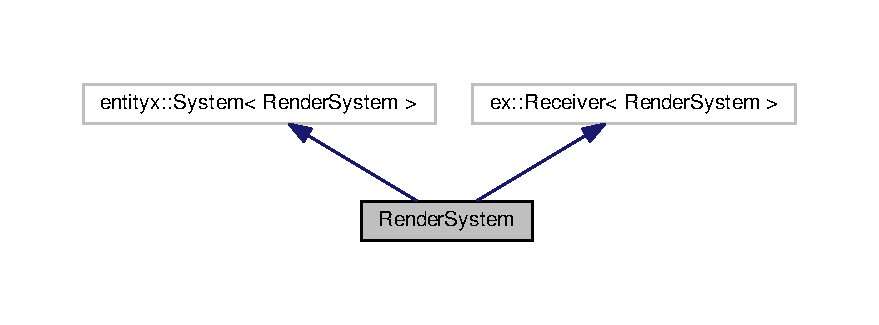
\includegraphics[width=350pt]{classRenderSystem__inherit__graph}
\end{center}
\end{figure}


Collaboration diagram for Render\+System\+:
\nopagebreak
\begin{figure}[H]
\begin{center}
\leavevmode
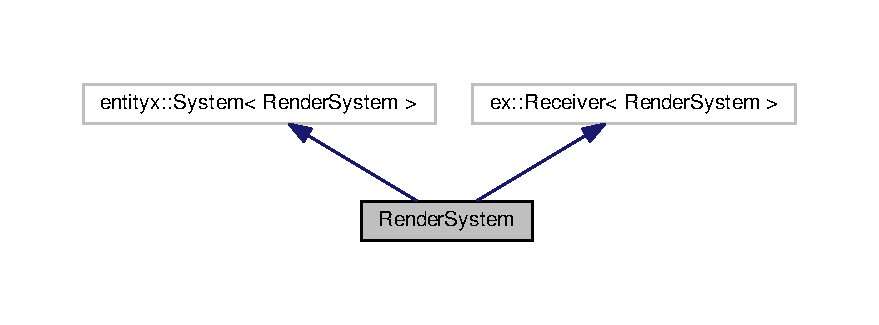
\includegraphics[width=350pt]{classRenderSystem__coll__graph}
\end{center}
\end{figure}
\subsection*{Public Member Functions}
\begin{DoxyCompactItemize}
\item 
\hyperlink{classRenderSystem_ac21b38b1afa0eb3d3f21f6d1db5c49ad}{Render\+System} (sf\+::\+Render\+Target \&target, sf\+::\+Font \&font)
\item 
void \hyperlink{classRenderSystem_aacda55df4d6fc4ffefdad3b38b4f25f8}{update} (ex\+::\+Entity\+Manager \&es, ex\+::\+Event\+Manager \&events, ex\+::\+Time\+Delta dt) override
\item 
void \hyperlink{classRenderSystem_a58134d130c3fbb29d5cb59bd0a9480ad}{configure} (ex\+::\+Event\+Manager \&events) override
\item 
void \hyperlink{classRenderSystem_af72a474303dbd088ef9b39983e9f6a64}{receive} (const \hyperlink{classEntitySpawnedEvent}{Entity\+Spawned\+Event} \&entity\+\_\+spawned\+\_\+event)
\item 
void \hyperlink{classRenderSystem_a82e833dc520c9fa822d66b3878c0de69}{receive} (const ex\+::\+Entity\+Destroyed\+Event \&entity\+\_\+destroyed\+\_\+event)
\item 
void \hyperlink{classRenderSystem_a4877dc8f72b552e4127628fd91e3a06d}{set\+Should\+Draw\+Pos} (bool flag)
\end{DoxyCompactItemize}


\subsection{Constructor \& Destructor Documentation}
\mbox{\Hypertarget{classRenderSystem_ac21b38b1afa0eb3d3f21f6d1db5c49ad}\label{classRenderSystem_ac21b38b1afa0eb3d3f21f6d1db5c49ad}} 
\index{Render\+System@{Render\+System}!Render\+System@{Render\+System}}
\index{Render\+System@{Render\+System}!Render\+System@{Render\+System}}
\subsubsection{\texorpdfstring{Render\+System()}{RenderSystem()}}
{\footnotesize\ttfamily Render\+System\+::\+Render\+System (\begin{DoxyParamCaption}\item[{sf\+::\+Render\+Target \&}]{target,  }\item[{sf\+::\+Font \&}]{font }\end{DoxyParamCaption})\hspace{0.3cm}{\ttfamily [explicit]}}



\subsection{Member Function Documentation}
\mbox{\Hypertarget{classRenderSystem_a58134d130c3fbb29d5cb59bd0a9480ad}\label{classRenderSystem_a58134d130c3fbb29d5cb59bd0a9480ad}} 
\index{Render\+System@{Render\+System}!configure@{configure}}
\index{configure@{configure}!Render\+System@{Render\+System}}
\subsubsection{\texorpdfstring{configure()}{configure()}}
{\footnotesize\ttfamily void Render\+System\+::configure (\begin{DoxyParamCaption}\item[{ex\+::\+Event\+Manager \&}]{events }\end{DoxyParamCaption})\hspace{0.3cm}{\ttfamily [override]}}

\mbox{\Hypertarget{classRenderSystem_af72a474303dbd088ef9b39983e9f6a64}\label{classRenderSystem_af72a474303dbd088ef9b39983e9f6a64}} 
\index{Render\+System@{Render\+System}!receive@{receive}}
\index{receive@{receive}!Render\+System@{Render\+System}}
\subsubsection{\texorpdfstring{receive()}{receive()}\hspace{0.1cm}{\footnotesize\ttfamily [1/2]}}
{\footnotesize\ttfamily void Render\+System\+::receive (\begin{DoxyParamCaption}\item[{const \hyperlink{classEntitySpawnedEvent}{Entity\+Spawned\+Event} \&}]{entity\+\_\+spawned\+\_\+event }\end{DoxyParamCaption})}

\mbox{\Hypertarget{classRenderSystem_a82e833dc520c9fa822d66b3878c0de69}\label{classRenderSystem_a82e833dc520c9fa822d66b3878c0de69}} 
\index{Render\+System@{Render\+System}!receive@{receive}}
\index{receive@{receive}!Render\+System@{Render\+System}}
\subsubsection{\texorpdfstring{receive()}{receive()}\hspace{0.1cm}{\footnotesize\ttfamily [2/2]}}
{\footnotesize\ttfamily void Render\+System\+::receive (\begin{DoxyParamCaption}\item[{const ex\+::\+Entity\+Destroyed\+Event \&}]{entity\+\_\+destroyed\+\_\+event }\end{DoxyParamCaption})}

\mbox{\Hypertarget{classRenderSystem_a4877dc8f72b552e4127628fd91e3a06d}\label{classRenderSystem_a4877dc8f72b552e4127628fd91e3a06d}} 
\index{Render\+System@{Render\+System}!set\+Should\+Draw\+Pos@{set\+Should\+Draw\+Pos}}
\index{set\+Should\+Draw\+Pos@{set\+Should\+Draw\+Pos}!Render\+System@{Render\+System}}
\subsubsection{\texorpdfstring{set\+Should\+Draw\+Pos()}{setShouldDrawPos()}}
{\footnotesize\ttfamily void Render\+System\+::set\+Should\+Draw\+Pos (\begin{DoxyParamCaption}\item[{bool}]{flag }\end{DoxyParamCaption})}

\mbox{\Hypertarget{classRenderSystem_aacda55df4d6fc4ffefdad3b38b4f25f8}\label{classRenderSystem_aacda55df4d6fc4ffefdad3b38b4f25f8}} 
\index{Render\+System@{Render\+System}!update@{update}}
\index{update@{update}!Render\+System@{Render\+System}}
\subsubsection{\texorpdfstring{update()}{update()}}
{\footnotesize\ttfamily void Render\+System\+::update (\begin{DoxyParamCaption}\item[{ex\+::\+Entity\+Manager \&}]{es,  }\item[{ex\+::\+Event\+Manager \&}]{events,  }\item[{ex\+::\+Time\+Delta}]{dt }\end{DoxyParamCaption})\hspace{0.3cm}{\ttfamily [override]}}



The documentation for this class was generated from the following files\+:\begin{DoxyCompactItemize}
\item 
systems/\hyperlink{render__system_8h}{render\+\_\+system.\+h}\item 
systems/\hyperlink{render__system_8cpp}{render\+\_\+system.\+cpp}\end{DoxyCompactItemize}

\hypertarget{classSpawnSystem}{}\section{Spawn\+System Class Reference}
\label{classSpawnSystem}\index{Spawn\+System@{Spawn\+System}}


{\ttfamily \#include $<$spawn\+\_\+system.\+h$>$}



Inheritance diagram for Spawn\+System\+:
\nopagebreak
\begin{figure}[H]
\begin{center}
\leavevmode
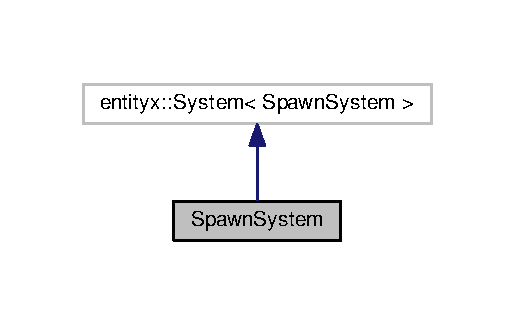
\includegraphics[width=247pt]{classSpawnSystem__inherit__graph}
\end{center}
\end{figure}


Collaboration diagram for Spawn\+System\+:
\nopagebreak
\begin{figure}[H]
\begin{center}
\leavevmode
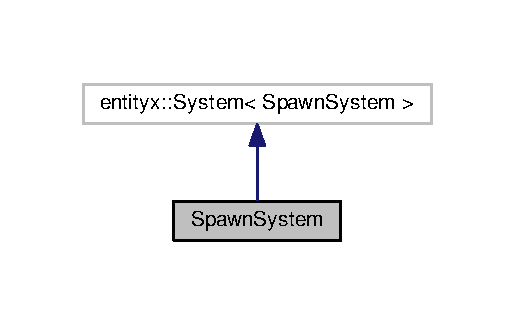
\includegraphics[width=247pt]{classSpawnSystem__coll__graph}
\end{center}
\end{figure}
\subsection*{Public Member Functions}
\begin{DoxyCompactItemize}
\item 
\hyperlink{classSpawnSystem_aa7a033d898d3f8c993ad0af84c635c0b}{Spawn\+System} (float width, float height, \hyperlink{spawn__system_8h_a2955cca9df1e3f8faa105a79669676dc}{Spawn\+Type} spawn\+\_\+type, int spawn\+\_\+count, int spawn\+\_\+speed=100)
\item 
void \hyperlink{classSpawnSystem_a881dab383c35a972c11bd4d8cff325a1}{update} (ex\+::\+Entity\+Manager \&es, ex\+::\+Event\+Manager \&events, ex\+::\+Time\+Delta dt) override
\end{DoxyCompactItemize}


\subsection{Constructor \& Destructor Documentation}
\mbox{\Hypertarget{classSpawnSystem_aa7a033d898d3f8c993ad0af84c635c0b}\label{classSpawnSystem_aa7a033d898d3f8c993ad0af84c635c0b}} 
\index{Spawn\+System@{Spawn\+System}!Spawn\+System@{Spawn\+System}}
\index{Spawn\+System@{Spawn\+System}!Spawn\+System@{Spawn\+System}}
\subsubsection{\texorpdfstring{Spawn\+System()}{SpawnSystem()}}
{\footnotesize\ttfamily Spawn\+System\+::\+Spawn\+System (\begin{DoxyParamCaption}\item[{float}]{width,  }\item[{float}]{height,  }\item[{\hyperlink{spawn__system_8h_a2955cca9df1e3f8faa105a79669676dc}{Spawn\+Type}}]{spawn\+\_\+type,  }\item[{int}]{spawn\+\_\+count,  }\item[{int}]{spawn\+\_\+speed = {\ttfamily 100} }\end{DoxyParamCaption})\hspace{0.3cm}{\ttfamily [inline]}, {\ttfamily [explicit]}}



\subsection{Member Function Documentation}
\mbox{\Hypertarget{classSpawnSystem_a881dab383c35a972c11bd4d8cff325a1}\label{classSpawnSystem_a881dab383c35a972c11bd4d8cff325a1}} 
\index{Spawn\+System@{Spawn\+System}!update@{update}}
\index{update@{update}!Spawn\+System@{Spawn\+System}}
\subsubsection{\texorpdfstring{update()}{update()}}
{\footnotesize\ttfamily void Spawn\+System\+::update (\begin{DoxyParamCaption}\item[{ex\+::\+Entity\+Manager \&}]{es,  }\item[{ex\+::\+Event\+Manager \&}]{events,  }\item[{ex\+::\+Time\+Delta}]{dt }\end{DoxyParamCaption})\hspace{0.3cm}{\ttfamily [inline]}, {\ttfamily [override]}}



The documentation for this class was generated from the following file\+:\begin{DoxyCompactItemize}
\item 
systems/\hyperlink{spawn__system_8h}{spawn\+\_\+system.\+h}\end{DoxyCompactItemize}

\chapter{File Documentation}
\hypertarget{common_8h}{}\section{common.\+h File Reference}
\label{common_8h}\index{common.\+h@{common.\+h}}
{\ttfamily \#include $<$entityx/entityx.\+h$>$}\newline
Include dependency graph for common.\+h\+:\nopagebreak
\begin{figure}[H]
\begin{center}
\leavevmode
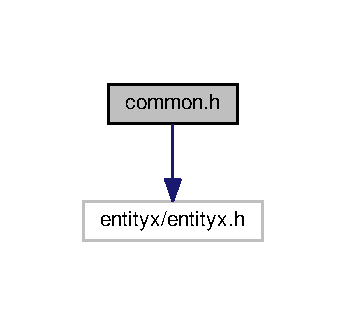
\includegraphics[width=166pt]{common_8h__incl}
\end{center}
\end{figure}
This graph shows which files directly or indirectly include this file\+:
\nopagebreak
\begin{figure}[H]
\begin{center}
\leavevmode
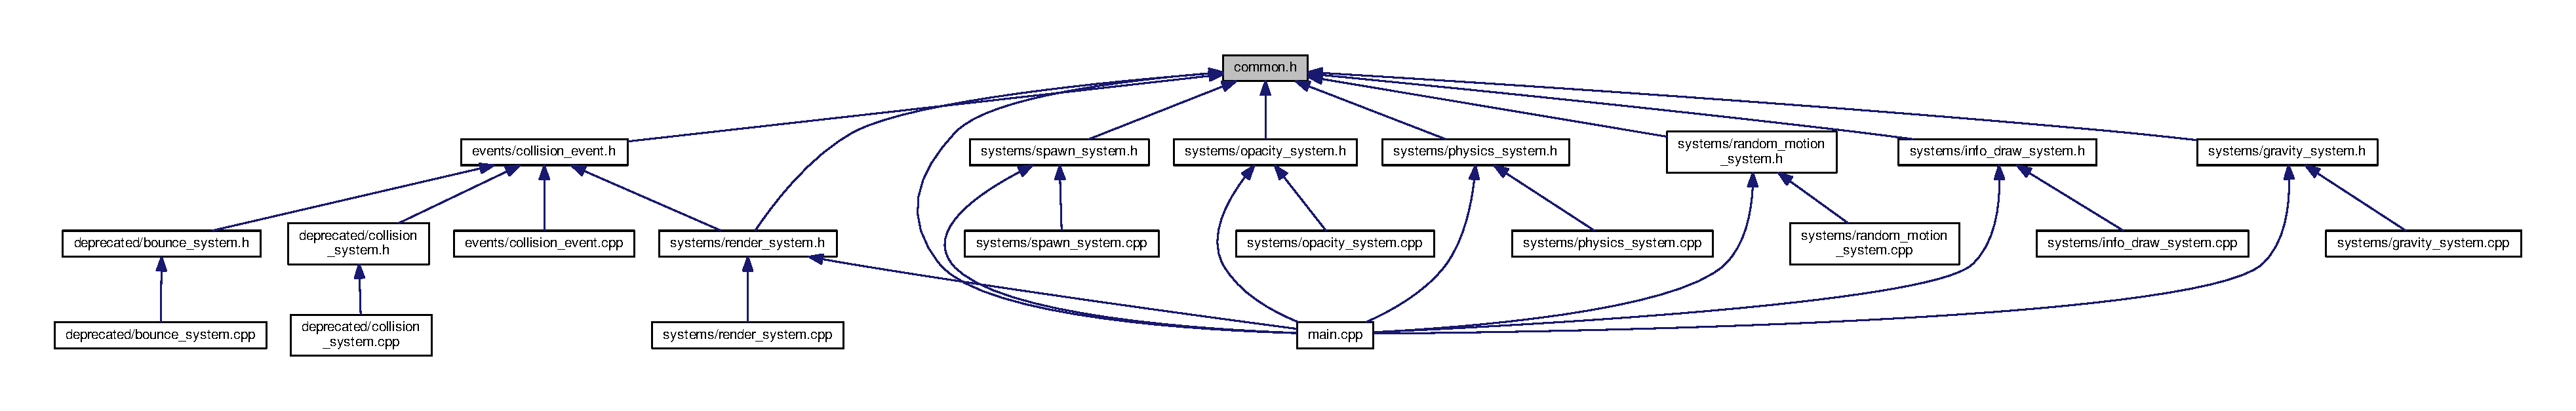
\includegraphics[width=350pt]{common_8h__dep__incl}
\end{center}
\end{figure}
\subsection*{Variables}
\begin{DoxyCompactItemize}
\item 
const float \hyperlink{common_8h_aeed5073a83bc94b5a7a797821fe60465}{P\+I\+X\+E\+L\+\_\+\+P\+E\+R\+\_\+\+M\+E\+T\+RE} = 50
\end{DoxyCompactItemize}


\subsection{Variable Documentation}
\mbox{\Hypertarget{common_8h_aeed5073a83bc94b5a7a797821fe60465}\label{common_8h_aeed5073a83bc94b5a7a797821fe60465}} 
\index{common.\+h@{common.\+h}!P\+I\+X\+E\+L\+\_\+\+P\+E\+R\+\_\+\+M\+E\+T\+RE@{P\+I\+X\+E\+L\+\_\+\+P\+E\+R\+\_\+\+M\+E\+T\+RE}}
\index{P\+I\+X\+E\+L\+\_\+\+P\+E\+R\+\_\+\+M\+E\+T\+RE@{P\+I\+X\+E\+L\+\_\+\+P\+E\+R\+\_\+\+M\+E\+T\+RE}!common.\+h@{common.\+h}}
\subsubsection{\texorpdfstring{P\+I\+X\+E\+L\+\_\+\+P\+E\+R\+\_\+\+M\+E\+T\+RE}{PIXEL\_PER\_METRE}}
{\footnotesize\ttfamily const float P\+I\+X\+E\+L\+\_\+\+P\+E\+R\+\_\+\+M\+E\+T\+RE = 50}


\hypertarget{body_8cpp}{}\section{components/body.cpp File Reference}
\label{body_8cpp}\index{components/body.\+cpp@{components/body.\+cpp}}
{\ttfamily \#include \char`\"{}body.\+h\char`\"{}}\newline
Include dependency graph for body.\+cpp\+:
\nopagebreak
\begin{figure}[H]
\begin{center}
\leavevmode
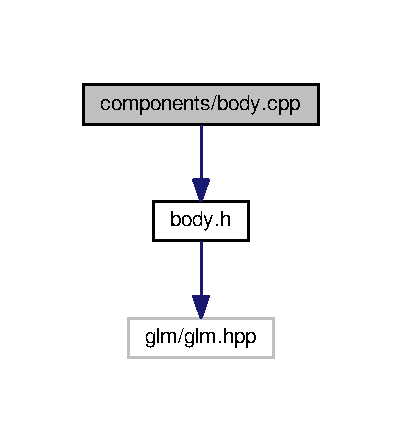
\includegraphics[width=193pt]{body_8cpp__incl}
\end{center}
\end{figure}

\hypertarget{body_8h}{}\section{components/body.h File Reference}
\label{body_8h}\index{components/body.\+h@{components/body.\+h}}
{\ttfamily \#include $<$glm/glm.\+hpp$>$}\newline
Include dependency graph for body.\+h\+:
\nopagebreak
\begin{figure}[H]
\begin{center}
\leavevmode
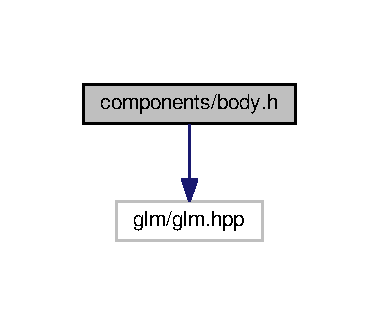
\includegraphics[width=182pt]{body_8h__incl}
\end{center}
\end{figure}
This graph shows which files directly or indirectly include this file\+:
\nopagebreak
\begin{figure}[H]
\begin{center}
\leavevmode
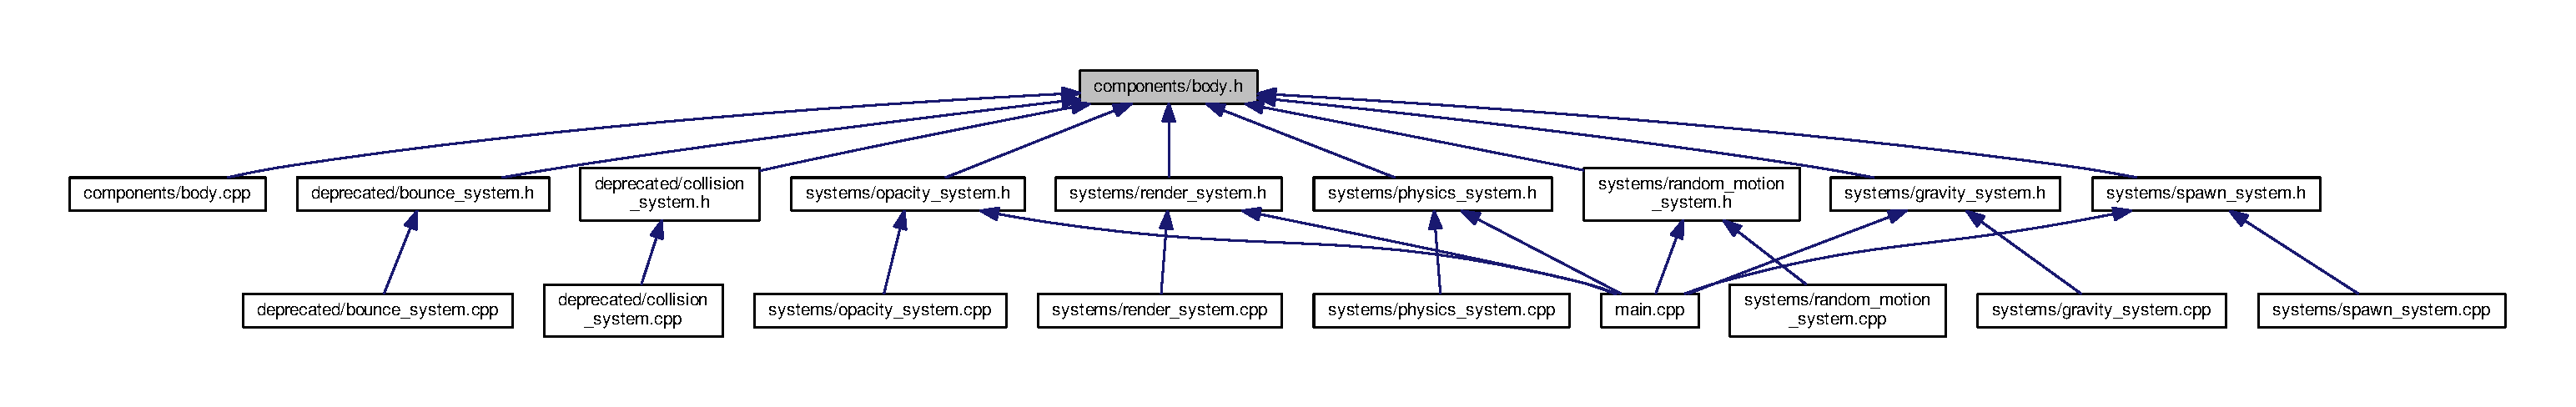
\includegraphics[width=350pt]{body_8h__dep__incl}
\end{center}
\end{figure}
\subsection*{Classes}
\begin{DoxyCompactItemize}
\item 
struct \hyperlink{structBody}{Body}
\end{DoxyCompactItemize}

\hypertarget{collideable_8cpp}{}\section{components/collideable.cpp File Reference}
\label{collideable_8cpp}\index{components/collideable.\+cpp@{components/collideable.\+cpp}}
{\ttfamily \#include \char`\"{}collideable.\+h\char`\"{}}\newline
Include dependency graph for collideable.\+cpp\+:
\nopagebreak
\begin{figure}[H]
\begin{center}
\leavevmode
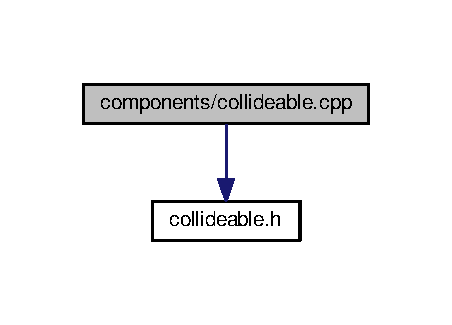
\includegraphics[width=217pt]{collideable_8cpp__incl}
\end{center}
\end{figure}

\hypertarget{collideable_8h}{}\section{components/collideable.h File Reference}
\label{collideable_8h}\index{components/collideable.\+h@{components/collideable.\+h}}
This graph shows which files directly or indirectly include this file\+:
\nopagebreak
\begin{figure}[H]
\begin{center}
\leavevmode
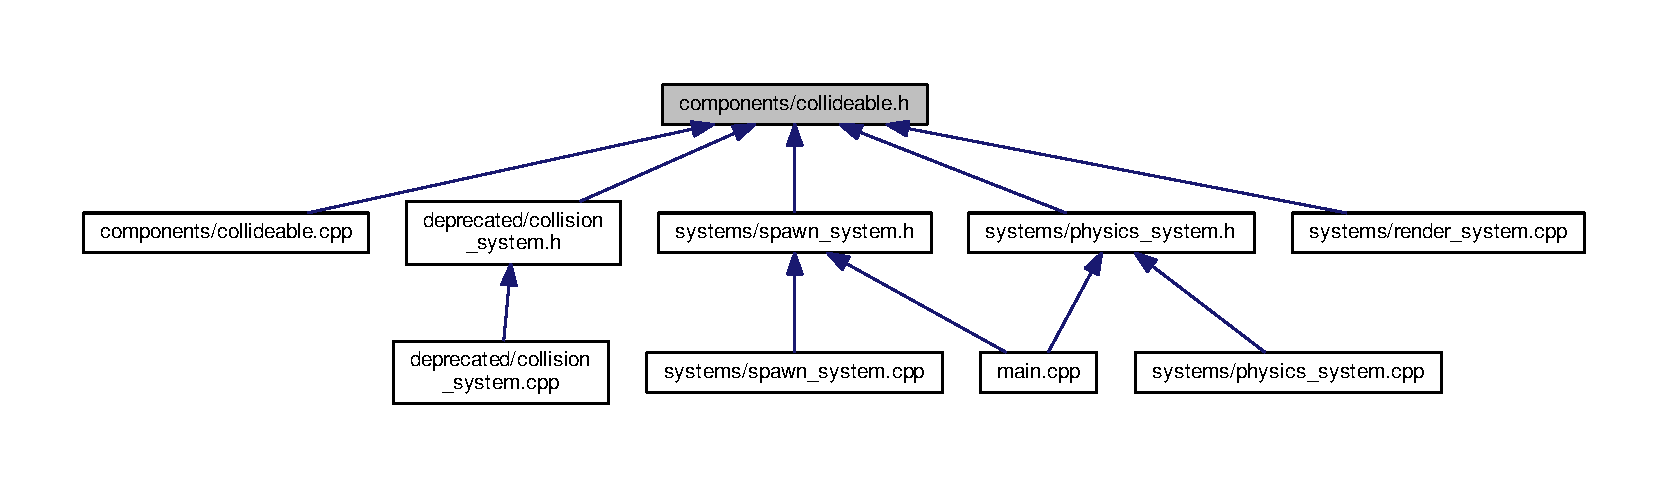
\includegraphics[width=350pt]{collideable_8h__dep__incl}
\end{center}
\end{figure}
\subsection*{Classes}
\begin{DoxyCompactItemize}
\item 
struct \hyperlink{structCollideable}{Collideable}
\end{DoxyCompactItemize}

\hypertarget{mass_8cpp}{}\section{components/mass.cpp File Reference}
\label{mass_8cpp}\index{components/mass.\+cpp@{components/mass.\+cpp}}
{\ttfamily \#include \char`\"{}mass.\+h\char`\"{}}\newline
Include dependency graph for mass.\+cpp\+:
\nopagebreak
\begin{figure}[H]
\begin{center}
\leavevmode
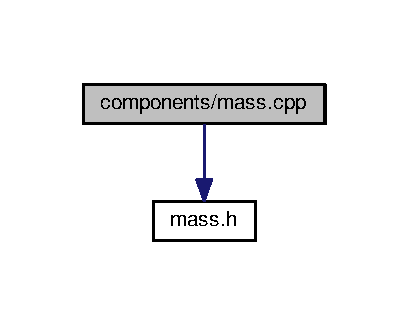
\includegraphics[width=196pt]{mass_8cpp__incl}
\end{center}
\end{figure}

\hypertarget{mass_8h}{}\section{components/mass.h File Reference}
\label{mass_8h}\index{components/mass.\+h@{components/mass.\+h}}
This graph shows which files directly or indirectly include this file\+:
\nopagebreak
\begin{figure}[H]
\begin{center}
\leavevmode
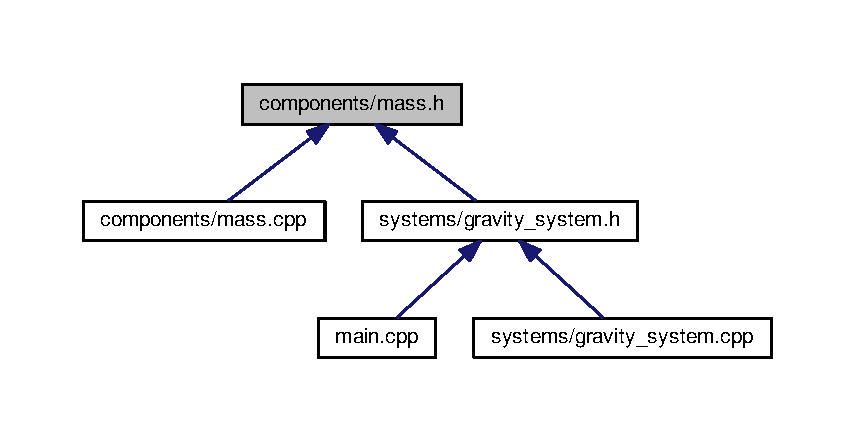
\includegraphics[width=350pt]{mass_8h__dep__incl}
\end{center}
\end{figure}
\subsection*{Classes}
\begin{DoxyCompactItemize}
\item 
class \hyperlink{classMass}{Mass}
\end{DoxyCompactItemize}

\hypertarget{renderable_8cpp}{}\section{components/renderable.cpp File Reference}
\label{renderable_8cpp}\index{components/renderable.\+cpp@{components/renderable.\+cpp}}
{\ttfamily \#include \char`\"{}renderable.\+h\char`\"{}}\newline
Include dependency graph for renderable.\+cpp\+:
\nopagebreak
\begin{figure}[H]
\begin{center}
\leavevmode
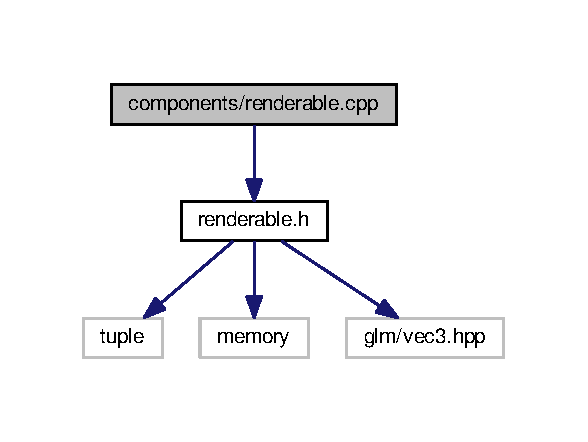
\includegraphics[width=282pt]{renderable_8cpp__incl}
\end{center}
\end{figure}

\hypertarget{renderable_8h}{}\section{components/renderable.h File Reference}
\label{renderable_8h}\index{components/renderable.\+h@{components/renderable.\+h}}
{\ttfamily \#include $<$tuple$>$}\newline
{\ttfamily \#include $<$memory$>$}\newline
{\ttfamily \#include $<$glm/vec3.\+hpp$>$}\newline
Include dependency graph for renderable.\+h\+:
\nopagebreak
\begin{figure}[H]
\begin{center}
\leavevmode
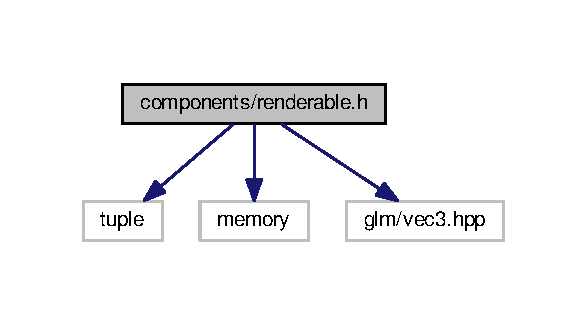
\includegraphics[width=282pt]{renderable_8h__incl}
\end{center}
\end{figure}
This graph shows which files directly or indirectly include this file\+:
\nopagebreak
\begin{figure}[H]
\begin{center}
\leavevmode
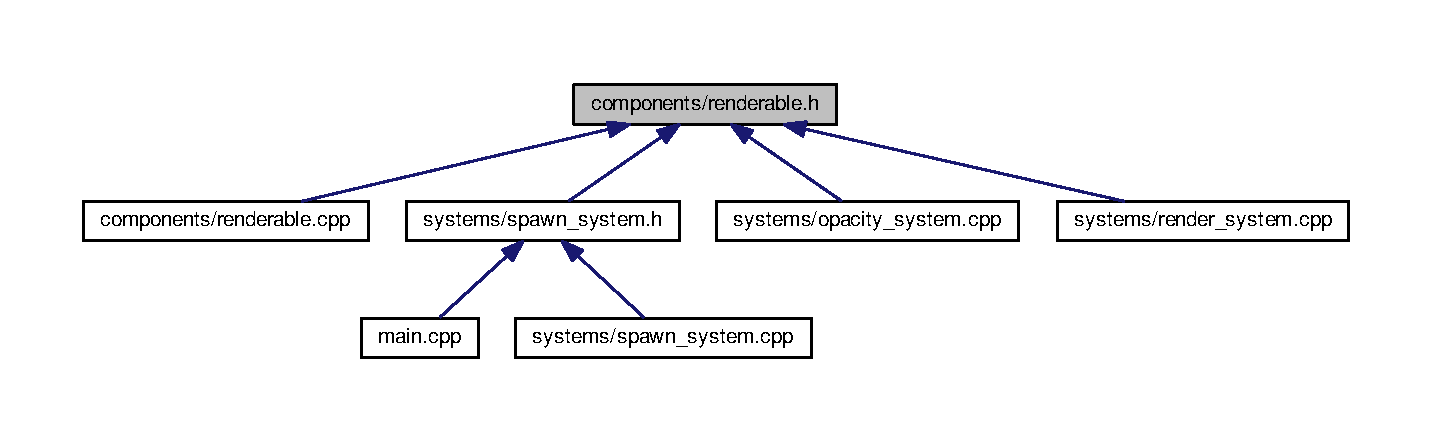
\includegraphics[width=350pt]{renderable_8h__dep__incl}
\end{center}
\end{figure}
\subsection*{Classes}
\begin{DoxyCompactItemize}
\item 
class \hyperlink{classRenderable}{Renderable}
\end{DoxyCompactItemize}
\subsection*{Typedefs}
\begin{DoxyCompactItemize}
\item 
typedef glm\+::uvec3 \hyperlink{renderable_8h_a81c9947aa4cb6db0d6522d01e75e6c30}{Color}
\end{DoxyCompactItemize}


\subsection{Typedef Documentation}
\mbox{\Hypertarget{renderable_8h_a81c9947aa4cb6db0d6522d01e75e6c30}\label{renderable_8h_a81c9947aa4cb6db0d6522d01e75e6c30}} 
\index{renderable.\+h@{renderable.\+h}!Color@{Color}}
\index{Color@{Color}!renderable.\+h@{renderable.\+h}}
\subsubsection{\texorpdfstring{Color}{Color}}
{\footnotesize\ttfamily typedef glm\+::uvec3 \hyperlink{renderable_8h_a81c9947aa4cb6db0d6522d01e75e6c30}{Color}}


\hypertarget{shapes_8cpp}{}\section{components/shapes.cpp File Reference}
\label{shapes_8cpp}\index{components/shapes.\+cpp@{components/shapes.\+cpp}}
{\ttfamily \#include \char`\"{}shapes.\+h\char`\"{}}\newline
Include dependency graph for shapes.\+cpp\+:
\nopagebreak
\begin{figure}[H]
\begin{center}
\leavevmode
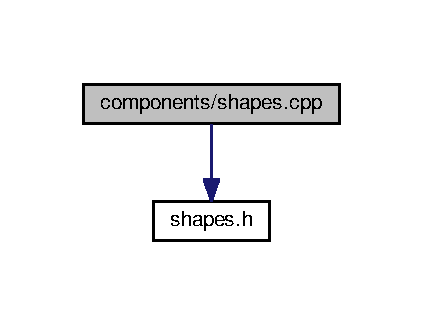
\includegraphics[width=203pt]{shapes_8cpp__incl}
\end{center}
\end{figure}

\hypertarget{shapes_8h}{}\section{components/shapes.h File Reference}
\label{shapes_8h}\index{components/shapes.\+h@{components/shapes.\+h}}
This graph shows which files directly or indirectly include this file\+:
\nopagebreak
\begin{figure}[H]
\begin{center}
\leavevmode
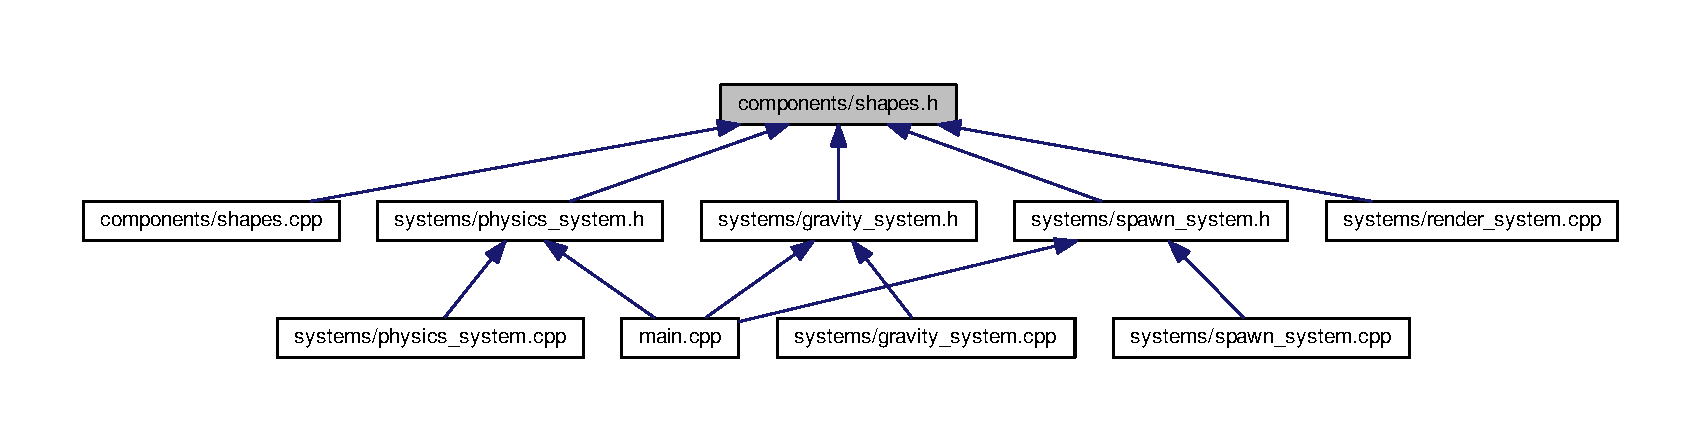
\includegraphics[width=350pt]{shapes_8h__dep__incl}
\end{center}
\end{figure}
\subsection*{Classes}
\begin{DoxyCompactItemize}
\item 
struct \hyperlink{structCircleShape}{Circle\+Shape}
\end{DoxyCompactItemize}

\hypertarget{bounce__system_8cpp}{}\section{deprecated/bounce\+\_\+system.cpp File Reference}
\label{bounce__system_8cpp}\index{deprecated/bounce\+\_\+system.\+cpp@{deprecated/bounce\+\_\+system.\+cpp}}
{\ttfamily \#include \char`\"{}bounce\+\_\+system.\+h\char`\"{}}\newline
Include dependency graph for bounce\+\_\+system.\+cpp\+:
\nopagebreak
\begin{figure}[H]
\begin{center}
\leavevmode
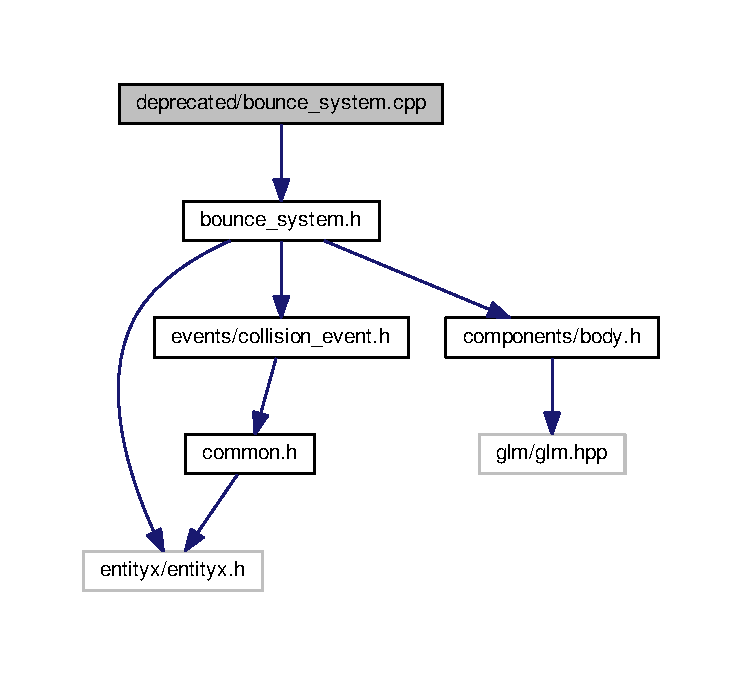
\includegraphics[width=350pt]{bounce__system_8cpp__incl}
\end{center}
\end{figure}

\hypertarget{bounce__system_8h}{}\section{deprecated/bounce\+\_\+system.h File Reference}
\label{bounce__system_8h}\index{deprecated/bounce\+\_\+system.\+h@{deprecated/bounce\+\_\+system.\+h}}
{\ttfamily \#include $<$entityx/entityx.\+h$>$}\newline
{\ttfamily \#include \char`\"{}events/collision\+\_\+event.\+h\char`\"{}}\newline
{\ttfamily \#include \char`\"{}components/body.\+h\char`\"{}}\newline
Include dependency graph for bounce\+\_\+system.\+h\+:
\nopagebreak
\begin{figure}[H]
\begin{center}
\leavevmode
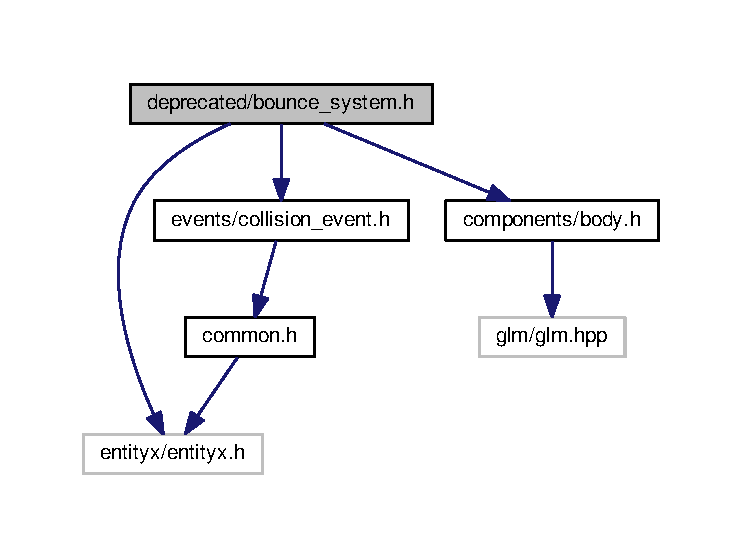
\includegraphics[width=350pt]{bounce__system_8h__incl}
\end{center}
\end{figure}
This graph shows which files directly or indirectly include this file\+:
\nopagebreak
\begin{figure}[H]
\begin{center}
\leavevmode
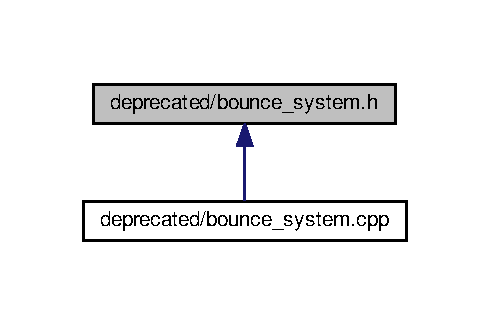
\includegraphics[width=235pt]{bounce__system_8h__dep__incl}
\end{center}
\end{figure}
\subsection*{Classes}
\begin{DoxyCompactItemize}
\item 
class \hyperlink{classBounceSystem}{Bounce\+System}
\end{DoxyCompactItemize}

\hypertarget{collision__system_8cpp}{}\section{deprecated/collision\+\_\+system.cpp File Reference}
\label{collision__system_8cpp}\index{deprecated/collision\+\_\+system.\+cpp@{deprecated/collision\+\_\+system.\+cpp}}
{\ttfamily \#include \char`\"{}collision\+\_\+system.\+h\char`\"{}}\newline
Include dependency graph for collision\+\_\+system.\+cpp\+:
\nopagebreak
\begin{figure}[H]
\begin{center}
\leavevmode
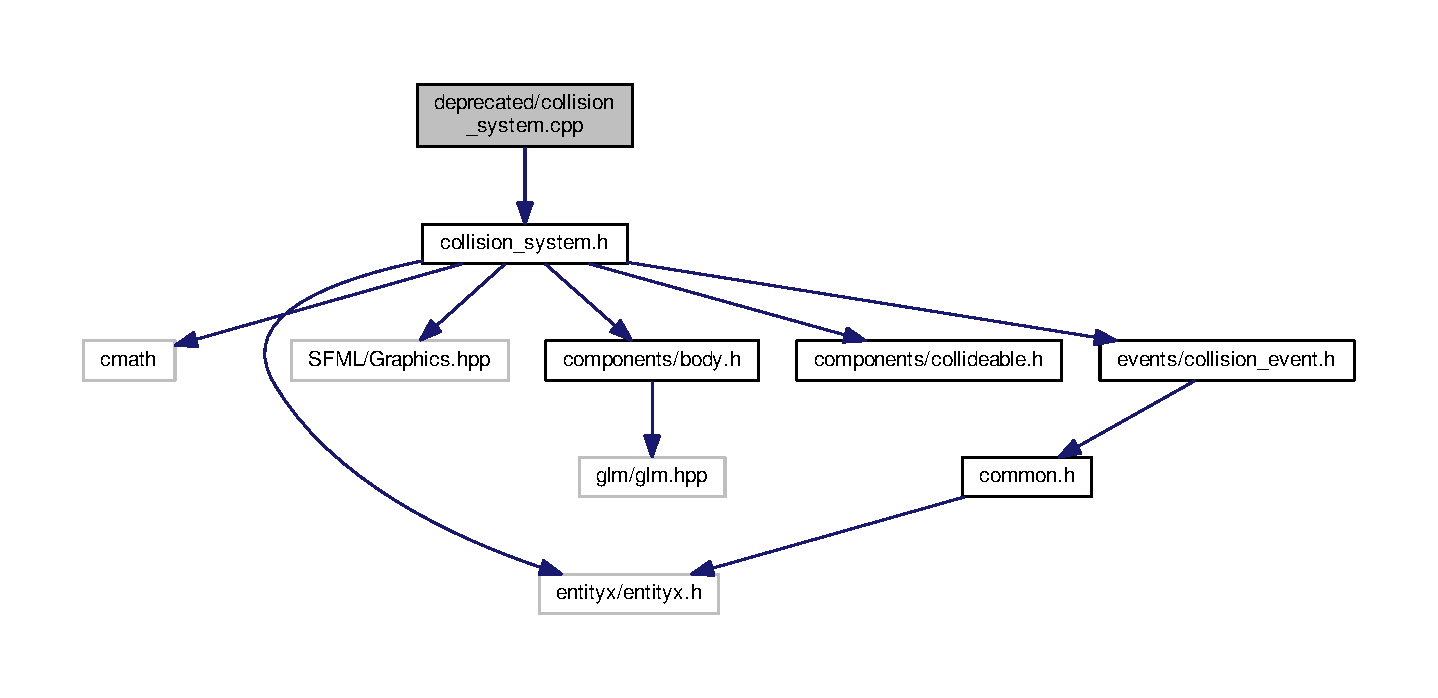
\includegraphics[width=350pt]{collision__system_8cpp__incl}
\end{center}
\end{figure}

\hypertarget{collision__system_8h}{}\section{deprecated/collision\+\_\+system.h File Reference}
\label{collision__system_8h}\index{deprecated/collision\+\_\+system.\+h@{deprecated/collision\+\_\+system.\+h}}
{\ttfamily \#include $<$cmath$>$}\newline
{\ttfamily \#include $<$entityx/entityx.\+h$>$}\newline
{\ttfamily \#include $<$S\+F\+M\+L/\+Graphics.\+hpp$>$}\newline
{\ttfamily \#include \char`\"{}components/body.\+h\char`\"{}}\newline
{\ttfamily \#include \char`\"{}components/collideable.\+h\char`\"{}}\newline
{\ttfamily \#include \char`\"{}events/collision\+\_\+event.\+h\char`\"{}}\newline
Include dependency graph for collision\+\_\+system.\+h\+:
\nopagebreak
\begin{figure}[H]
\begin{center}
\leavevmode
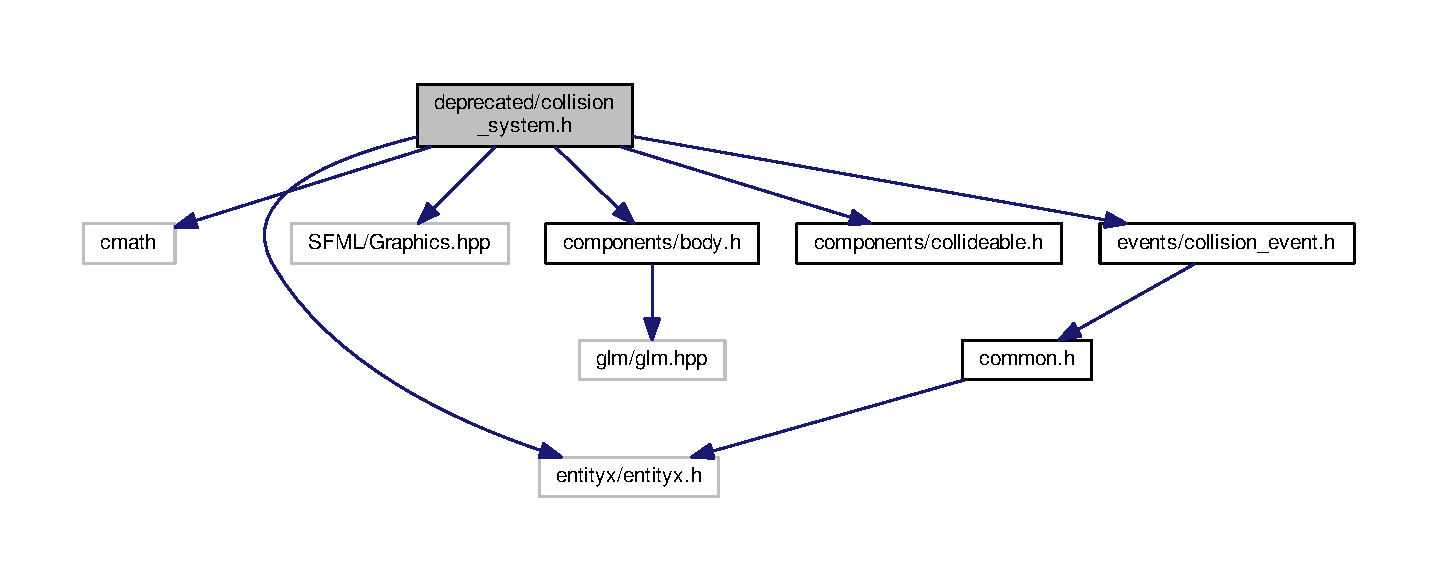
\includegraphics[width=350pt]{collision__system_8h__incl}
\end{center}
\end{figure}
This graph shows which files directly or indirectly include this file\+:
\nopagebreak
\begin{figure}[H]
\begin{center}
\leavevmode
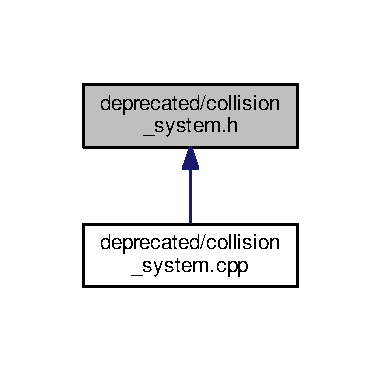
\includegraphics[width=183pt]{collision__system_8h__dep__incl}
\end{center}
\end{figure}
\subsection*{Classes}
\begin{DoxyCompactItemize}
\item 
class \hyperlink{classCollisionSystem}{Collision\+System}
\end{DoxyCompactItemize}

\hypertarget{collision__event_8cpp}{}\section{events/collision\+\_\+event.cpp File Reference}
\label{collision__event_8cpp}\index{events/collision\+\_\+event.\+cpp@{events/collision\+\_\+event.\+cpp}}
{\ttfamily \#include \char`\"{}collision\+\_\+event.\+h\char`\"{}}\newline
Include dependency graph for collision\+\_\+event.\+cpp\+:
\nopagebreak
\begin{figure}[H]
\begin{center}
\leavevmode
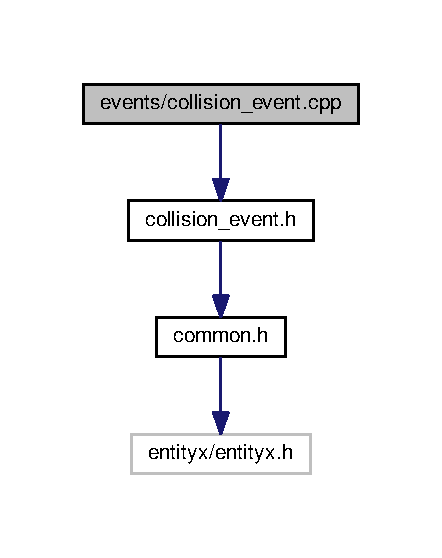
\includegraphics[width=212pt]{collision__event_8cpp__incl}
\end{center}
\end{figure}

\hypertarget{collision__event_8h}{}\section{events/collision\+\_\+event.h File Reference}
\label{collision__event_8h}\index{events/collision\+\_\+event.\+h@{events/collision\+\_\+event.\+h}}
{\ttfamily \#include \char`\"{}common.\+h\char`\"{}}\newline
Include dependency graph for collision\+\_\+event.\+h\+:
\nopagebreak
\begin{figure}[H]
\begin{center}
\leavevmode
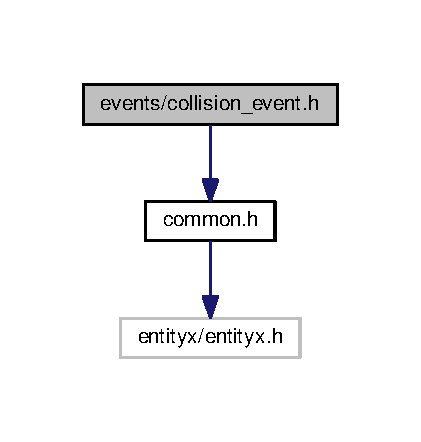
\includegraphics[width=202pt]{collision__event_8h__incl}
\end{center}
\end{figure}
This graph shows which files directly or indirectly include this file\+:
\nopagebreak
\begin{figure}[H]
\begin{center}
\leavevmode
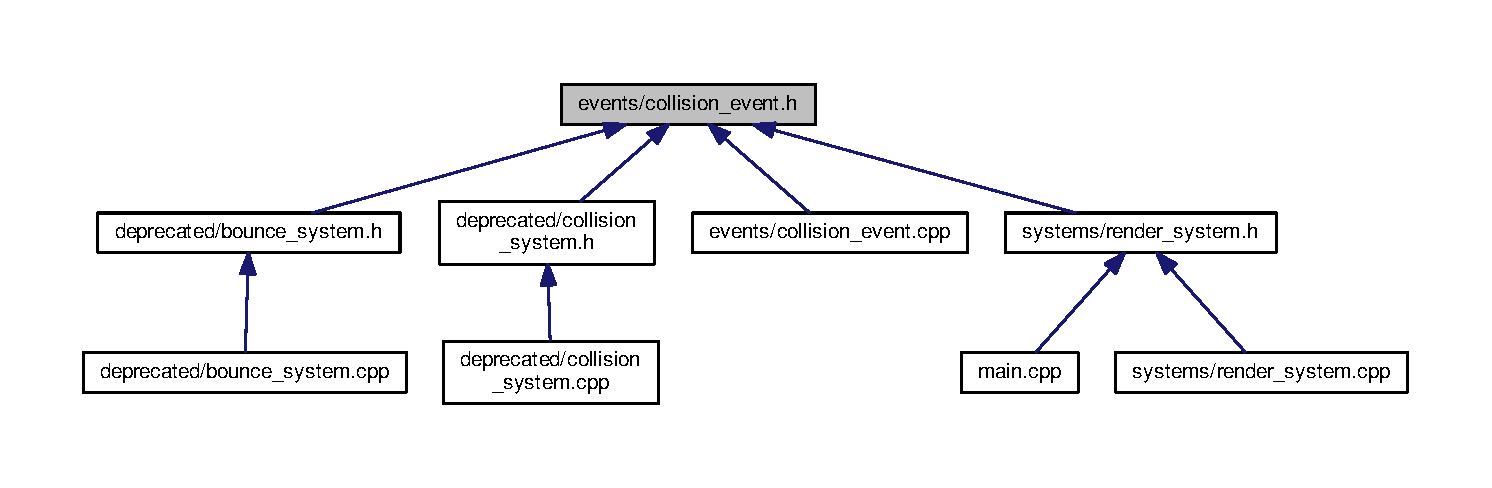
\includegraphics[width=350pt]{collision__event_8h__dep__incl}
\end{center}
\end{figure}
\subsection*{Classes}
\begin{DoxyCompactItemize}
\item 
struct \hyperlink{structCollisionEvent}{Collision\+Event}
\end{DoxyCompactItemize}

\hypertarget{EntitySpawnedEvent_8cpp}{}\section{events/\+Entity\+Spawned\+Event.cpp File Reference}
\label{EntitySpawnedEvent_8cpp}\index{events/\+Entity\+Spawned\+Event.\+cpp@{events/\+Entity\+Spawned\+Event.\+cpp}}
{\ttfamily \#include \char`\"{}Entity\+Spawned\+Event.\+h\char`\"{}}\newline
Include dependency graph for Entity\+Spawned\+Event.\+cpp\+:
\nopagebreak
\begin{figure}[H]
\begin{center}
\leavevmode
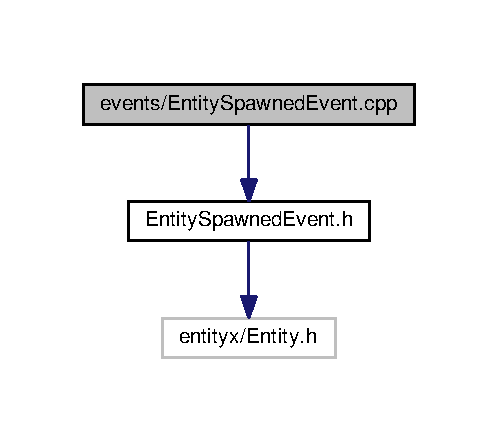
\includegraphics[width=239pt]{EntitySpawnedEvent_8cpp__incl}
\end{center}
\end{figure}

\hypertarget{EntitySpawnedEvent_8h}{}\section{events/\+Entity\+Spawned\+Event.h File Reference}
\label{EntitySpawnedEvent_8h}\index{events/\+Entity\+Spawned\+Event.\+h@{events/\+Entity\+Spawned\+Event.\+h}}
{\ttfamily \#include $<$entityx/\+Entity.\+h$>$}\newline
Include dependency graph for Entity\+Spawned\+Event.\+h\+:
\nopagebreak
\begin{figure}[H]
\begin{center}
\leavevmode
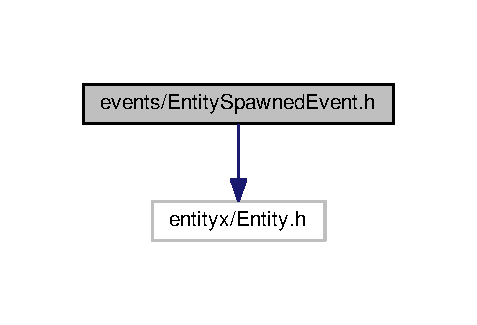
\includegraphics[width=229pt]{EntitySpawnedEvent_8h__incl}
\end{center}
\end{figure}
This graph shows which files directly or indirectly include this file\+:
\nopagebreak
\begin{figure}[H]
\begin{center}
\leavevmode
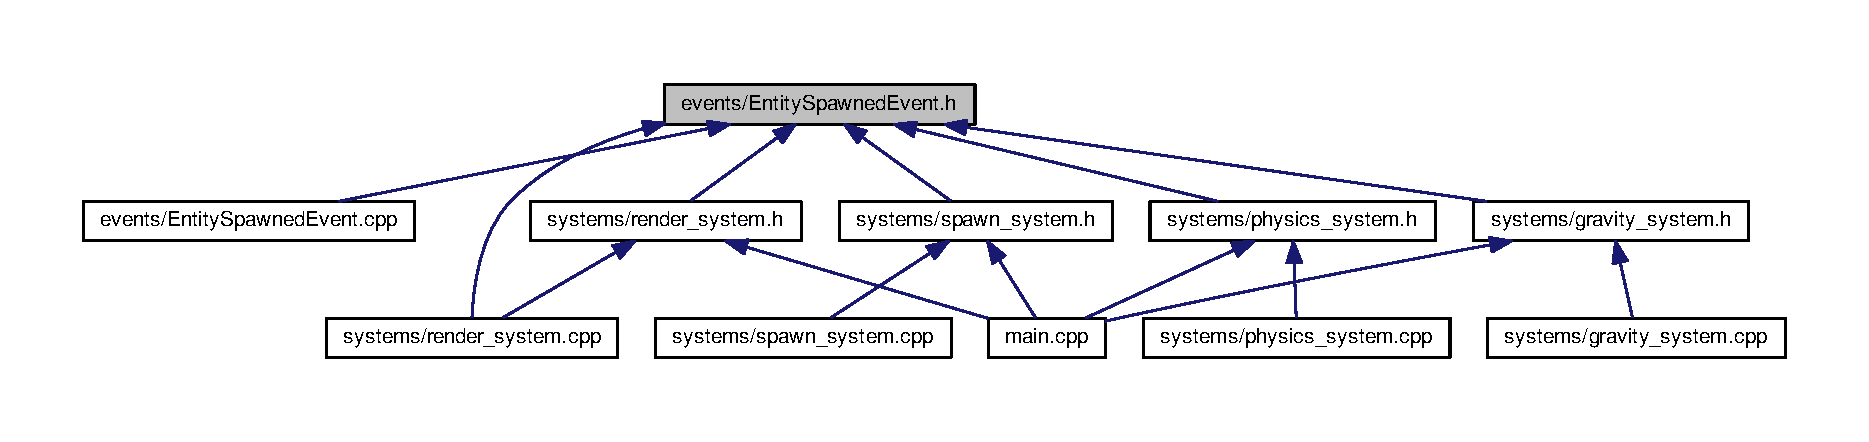
\includegraphics[width=350pt]{EntitySpawnedEvent_8h__dep__incl}
\end{center}
\end{figure}
\subsection*{Classes}
\begin{DoxyCompactItemize}
\item 
class \hyperlink{classEntitySpawnedEvent}{Entity\+Spawned\+Event}
\end{DoxyCompactItemize}

\hypertarget{main_8cpp}{}\section{main.\+cpp File Reference}
\label{main_8cpp}\index{main.\+cpp@{main.\+cpp}}
{\ttfamily \#include \char`\"{}systems/spawn\+\_\+system.\+h\char`\"{}}\newline
{\ttfamily \#include \char`\"{}systems/opacity\+\_\+system.\+h\char`\"{}}\newline
{\ttfamily \#include \char`\"{}systems/render\+\_\+system.\+h\char`\"{}}\newline
{\ttfamily \#include \char`\"{}systems/physics\+\_\+system.\+h\char`\"{}}\newline
{\ttfamily \#include \char`\"{}systems/random\+\_\+motion\+\_\+system.\+h\char`\"{}}\newline
{\ttfamily \#include \char`\"{}systems/info\+\_\+draw\+\_\+system.\+h\char`\"{}}\newline
{\ttfamily \#include \char`\"{}systems/gravity\+\_\+system.\+h\char`\"{}}\newline
{\ttfamily \#include \char`\"{}common.\+h\char`\"{}}\newline
{\ttfamily \#include $<$S\+F\+M\+L/\+Window.\+hpp$>$}\newline
{\ttfamily \#include $<$entityx/entityx.\+h$>$}\newline
Include dependency graph for main.\+cpp\+:
\nopagebreak
\begin{figure}[H]
\begin{center}
\leavevmode
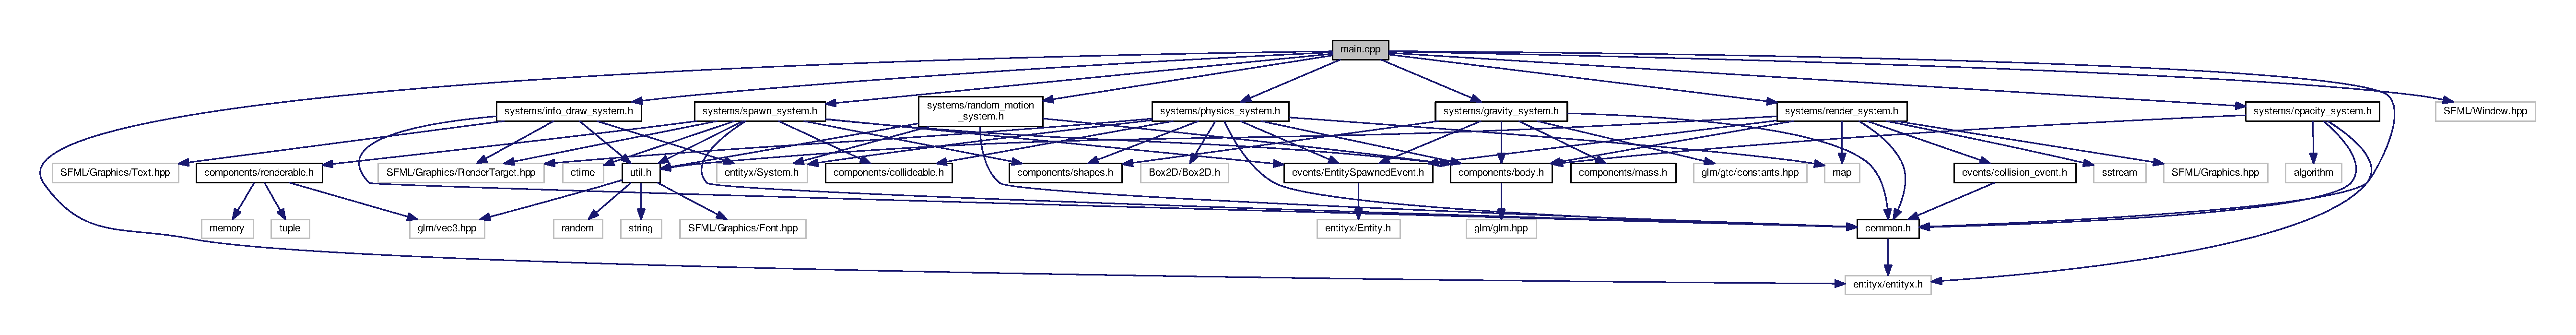
\includegraphics[width=350pt]{main_8cpp__incl}
\end{center}
\end{figure}
\subsection*{Classes}
\begin{DoxyCompactItemize}
\item 
class \hyperlink{classEcsManager}{Ecs\+Manager}
\end{DoxyCompactItemize}
\subsection*{Functions}
\begin{DoxyCompactItemize}
\item 
int \hyperlink{main_8cpp_ae66f6b31b5ad750f1fe042a706a4e3d4}{main} ()
\end{DoxyCompactItemize}


\subsection{Function Documentation}
\mbox{\Hypertarget{main_8cpp_ae66f6b31b5ad750f1fe042a706a4e3d4}\label{main_8cpp_ae66f6b31b5ad750f1fe042a706a4e3d4}} 
\index{main.\+cpp@{main.\+cpp}!main@{main}}
\index{main@{main}!main.\+cpp@{main.\+cpp}}
\subsubsection{\texorpdfstring{main()}{main()}}
{\footnotesize\ttfamily int main (\begin{DoxyParamCaption}{ }\end{DoxyParamCaption})}


\hypertarget{gravity__system_8cpp}{}\section{systems/gravity\+\_\+system.cpp File Reference}
\label{gravity__system_8cpp}\index{systems/gravity\+\_\+system.\+cpp@{systems/gravity\+\_\+system.\+cpp}}
{\ttfamily \#include \char`\"{}gravity\+\_\+system.\+h\char`\"{}}\newline
Include dependency graph for gravity\+\_\+system.\+cpp\+:
\nopagebreak
\begin{figure}[H]
\begin{center}
\leavevmode
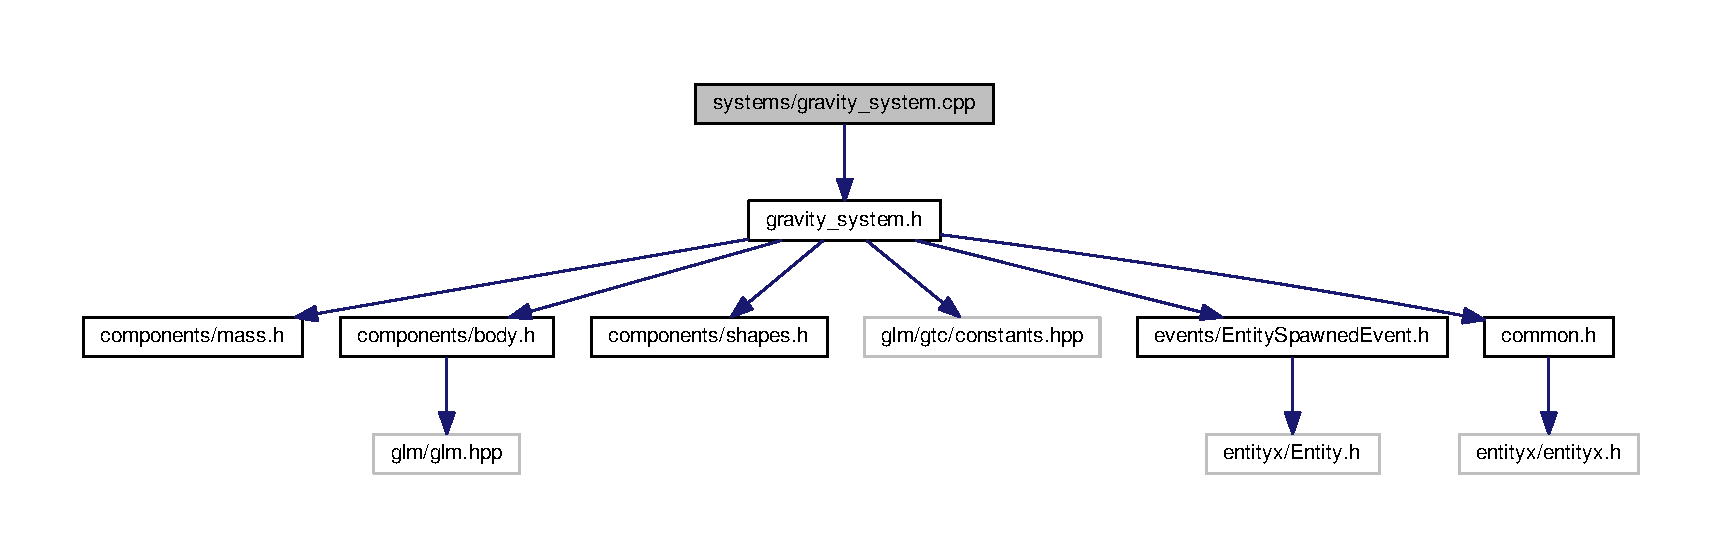
\includegraphics[width=350pt]{gravity__system_8cpp__incl}
\end{center}
\end{figure}

\hypertarget{gravity__system_8h}{}\section{systems/gravity\+\_\+system.h File Reference}
\label{gravity__system_8h}\index{systems/gravity\+\_\+system.\+h@{systems/gravity\+\_\+system.\+h}}
{\ttfamily \#include $<$components/mass.\+h$>$}\newline
{\ttfamily \#include $<$components/body.\+h$>$}\newline
{\ttfamily \#include $<$components/shapes.\+h$>$}\newline
{\ttfamily \#include $<$glm/gtc/constants.\+hpp$>$}\newline
{\ttfamily \#include \char`\"{}events/\+Entity\+Spawned\+Event.\+h\char`\"{}}\newline
{\ttfamily \#include \char`\"{}common.\+h\char`\"{}}\newline
Include dependency graph for gravity\+\_\+system.\+h\+:
\nopagebreak
\begin{figure}[H]
\begin{center}
\leavevmode
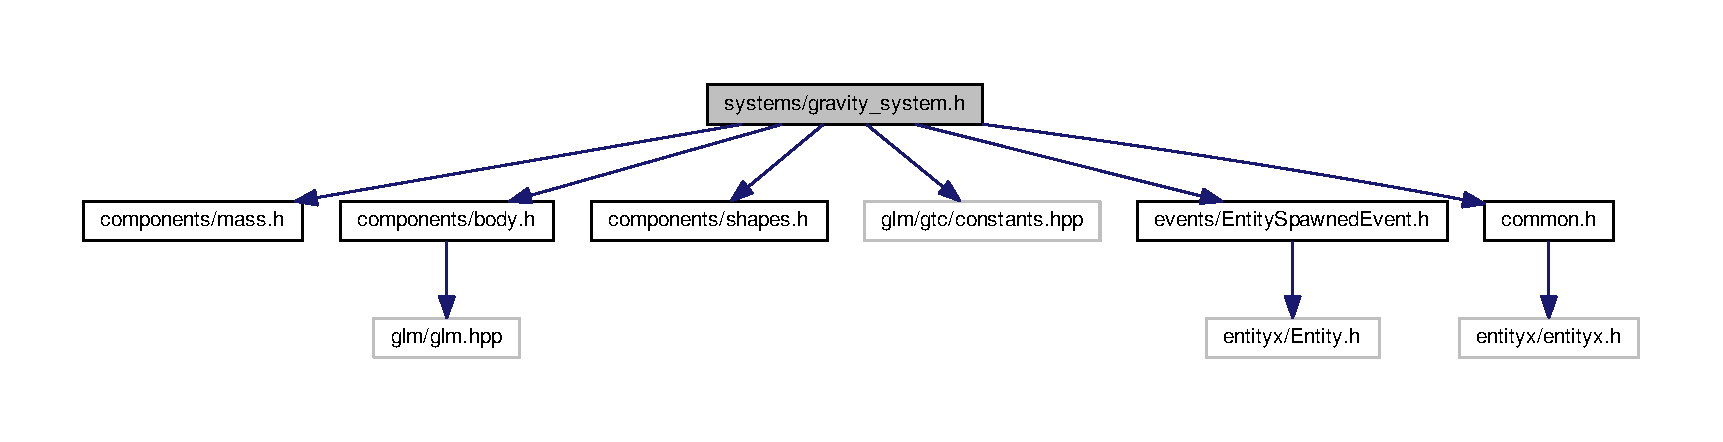
\includegraphics[width=350pt]{gravity__system_8h__incl}
\end{center}
\end{figure}
This graph shows which files directly or indirectly include this file\+:
\nopagebreak
\begin{figure}[H]
\begin{center}
\leavevmode
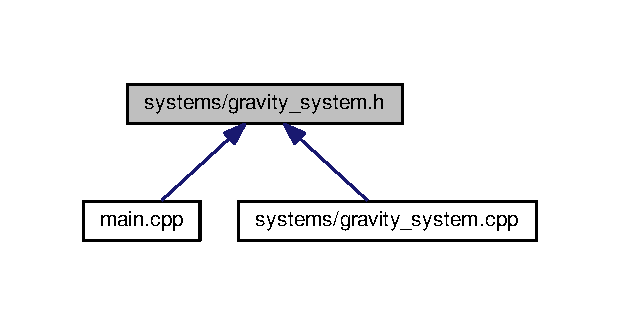
\includegraphics[width=298pt]{gravity__system_8h__dep__incl}
\end{center}
\end{figure}
\subsection*{Classes}
\begin{DoxyCompactItemize}
\item 
class \hyperlink{classGravitySystem}{Gravity\+System}
\end{DoxyCompactItemize}

\hypertarget{info__draw__system_8cpp}{}\section{systems/info\+\_\+draw\+\_\+system.cpp File Reference}
\label{info__draw__system_8cpp}\index{systems/info\+\_\+draw\+\_\+system.\+cpp@{systems/info\+\_\+draw\+\_\+system.\+cpp}}
{\ttfamily \#include $<$sstream$>$}\newline
{\ttfamily \#include \char`\"{}info\+\_\+draw\+\_\+system.\+h\char`\"{}}\newline
Include dependency graph for info\+\_\+draw\+\_\+system.\+cpp\+:
\nopagebreak
\begin{figure}[H]
\begin{center}
\leavevmode
\includegraphics[width=350pt]{info__draw__system_8cpp__incl}
\end{center}
\end{figure}

\hypertarget{info__draw__system_8h}{}\section{systems/info\+\_\+draw\+\_\+system.h File Reference}
\label{info__draw__system_8h}\index{systems/info\+\_\+draw\+\_\+system.\+h@{systems/info\+\_\+draw\+\_\+system.\+h}}
{\ttfamily \#include $<$entityx/\+System.\+h$>$}\newline
{\ttfamily \#include $<$S\+F\+M\+L/\+Graphics/\+Text.\+hpp$>$}\newline
{\ttfamily \#include $<$S\+F\+M\+L/\+Graphics/\+Render\+Target.\+hpp$>$}\newline
{\ttfamily \#include \char`\"{}util.\+h\char`\"{}}\newline
{\ttfamily \#include \char`\"{}common.\+h\char`\"{}}\newline
Include dependency graph for info\+\_\+draw\+\_\+system.\+h\+:
\nopagebreak
\begin{figure}[H]
\begin{center}
\leavevmode
\includegraphics[width=350pt]{info__draw__system_8h__incl}
\end{center}
\end{figure}
This graph shows which files directly or indirectly include this file\+:
\nopagebreak
\begin{figure}[H]
\begin{center}
\leavevmode
\includegraphics[width=310pt]{info__draw__system_8h__dep__incl}
\end{center}
\end{figure}
\subsection*{Classes}
\begin{DoxyCompactItemize}
\item 
class \hyperlink{classInfoDrawSystem}{Info\+Draw\+System}
\end{DoxyCompactItemize}

\hypertarget{opacity__system_8cpp}{}\section{systems/opacity\+\_\+system.cpp File Reference}
\label{opacity__system_8cpp}\index{systems/opacity\+\_\+system.\+cpp@{systems/opacity\+\_\+system.\+cpp}}
{\ttfamily \#include \char`\"{}opacity\+\_\+system.\+h\char`\"{}}\newline
{\ttfamily \#include \char`\"{}components/renderable.\+h\char`\"{}}\newline
Include dependency graph for opacity\+\_\+system.\+cpp\+:
\nopagebreak
\begin{figure}[H]
\begin{center}
\leavevmode
\includegraphics[width=350pt]{opacity__system_8cpp__incl}
\end{center}
\end{figure}

\hypertarget{opacity__system_8h}{}\section{systems/opacity\+\_\+system.h File Reference}
\label{opacity__system_8h}\index{systems/opacity\+\_\+system.\+h@{systems/opacity\+\_\+system.\+h}}
{\ttfamily \#include $<$algorithm$>$}\newline
{\ttfamily \#include $<$entityx/entityx.\+h$>$}\newline
{\ttfamily \#include \char`\"{}components/body.\+h\char`\"{}}\newline
{\ttfamily \#include \char`\"{}common.\+h\char`\"{}}\newline
Include dependency graph for opacity\+\_\+system.\+h\+:
\nopagebreak
\begin{figure}[H]
\begin{center}
\leavevmode
\includegraphics[width=350pt]{opacity__system_8h__incl}
\end{center}
\end{figure}
This graph shows which files directly or indirectly include this file\+:
\nopagebreak
\begin{figure}[H]
\begin{center}
\leavevmode
\includegraphics[width=300pt]{opacity__system_8h__dep__incl}
\end{center}
\end{figure}
\subsection*{Classes}
\begin{DoxyCompactItemize}
\item 
struct \hyperlink{structOpacitySystem}{Opacity\+System}
\end{DoxyCompactItemize}

\hypertarget{physics__system_8cpp}{}\section{systems/physics\+\_\+system.cpp File Reference}
\label{physics__system_8cpp}\index{systems/physics\+\_\+system.\+cpp@{systems/physics\+\_\+system.\+cpp}}
{\ttfamily \#include \char`\"{}physics\+\_\+system.\+h\char`\"{}}\newline
Include dependency graph for physics\+\_\+system.\+cpp\+:
\nopagebreak
\begin{figure}[H]
\begin{center}
\leavevmode
\includegraphics[width=350pt]{physics__system_8cpp__incl}
\end{center}
\end{figure}

\hypertarget{physics__system_8h}{}\section{systems/physics\+\_\+system.h File Reference}
\label{physics__system_8h}\index{systems/physics\+\_\+system.\+h@{systems/physics\+\_\+system.\+h}}
{\ttfamily \#include $<$entityx/\+System.\+h$>$}\newline
{\ttfamily \#include $<$Box2\+D/\+Box2\+D.\+h$>$}\newline
{\ttfamily \#include $<$map$>$}\newline
{\ttfamily \#include $<$S\+F\+M\+L/\+Graphics/\+Render\+Target.\+hpp$>$}\newline
{\ttfamily \#include $<$components/shapes.\+h$>$}\newline
{\ttfamily \#include $<$components/collideable.\+h$>$}\newline
{\ttfamily \#include \char`\"{}components/body.\+h\char`\"{}}\newline
{\ttfamily \#include \char`\"{}events/\+Entity\+Spawned\+Event.\+h\char`\"{}}\newline
{\ttfamily \#include \char`\"{}common.\+h\char`\"{}}\newline
Include dependency graph for physics\+\_\+system.\+h\+:
\nopagebreak
\begin{figure}[H]
\begin{center}
\leavevmode
\includegraphics[width=350pt]{physics__system_8h__incl}
\end{center}
\end{figure}
This graph shows which files directly or indirectly include this file\+:
\nopagebreak
\begin{figure}[H]
\begin{center}
\leavevmode
\includegraphics[width=302pt]{physics__system_8h__dep__incl}
\end{center}
\end{figure}
\subsection*{Classes}
\begin{DoxyCompactItemize}
\item 
class \hyperlink{classPhysicsSystem}{Physics\+System}
\end{DoxyCompactItemize}

\hypertarget{random__motion__system_8cpp}{}\section{systems/random\+\_\+motion\+\_\+system.cpp File Reference}
\label{random__motion__system_8cpp}\index{systems/random\+\_\+motion\+\_\+system.\+cpp@{systems/random\+\_\+motion\+\_\+system.\+cpp}}
{\ttfamily \#include \char`\"{}random\+\_\+motion\+\_\+system.\+h\char`\"{}}\newline
Include dependency graph for random\+\_\+motion\+\_\+system.\+cpp\+:
\nopagebreak
\begin{figure}[H]
\begin{center}
\leavevmode
\includegraphics[width=350pt]{random__motion__system_8cpp__incl}
\end{center}
\end{figure}

\hypertarget{random__motion__system_8h}{}\section{systems/random\+\_\+motion\+\_\+system.h File Reference}
\label{random__motion__system_8h}\index{systems/random\+\_\+motion\+\_\+system.\+h@{systems/random\+\_\+motion\+\_\+system.\+h}}
{\ttfamily \#include $<$entityx/\+System.\+h$>$}\newline
{\ttfamily \#include \char`\"{}components/body.\+h\char`\"{}}\newline
{\ttfamily \#include \char`\"{}common.\+h\char`\"{}}\newline
{\ttfamily \#include \char`\"{}util.\+h\char`\"{}}\newline
Include dependency graph for random\+\_\+motion\+\_\+system.\+h\+:
\nopagebreak
\begin{figure}[H]
\begin{center}
\leavevmode
\includegraphics[width=350pt]{random__motion__system_8h__incl}
\end{center}
\end{figure}
This graph shows which files directly or indirectly include this file\+:
\nopagebreak
\begin{figure}[H]
\begin{center}
\leavevmode
\includegraphics[width=278pt]{random__motion__system_8h__dep__incl}
\end{center}
\end{figure}
\subsection*{Classes}
\begin{DoxyCompactItemize}
\item 
class \hyperlink{classRandomMotionSystem}{Random\+Motion\+System}
\end{DoxyCompactItemize}

\hypertarget{render__system_8cpp}{}\section{systems/render\+\_\+system.cpp File Reference}
\label{render__system_8cpp}\index{systems/render\+\_\+system.\+cpp@{systems/render\+\_\+system.\+cpp}}
{\ttfamily \#include \char`\"{}render\+\_\+system.\+h\char`\"{}}\newline
{\ttfamily \#include \char`\"{}events/\+Entity\+Spawned\+Event.\+h\char`\"{}}\newline
{\ttfamily \#include \char`\"{}components/collideable.\+h\char`\"{}}\newline
{\ttfamily \#include \char`\"{}util.\+h\char`\"{}}\newline
{\ttfamily \#include \char`\"{}components/renderable.\+h\char`\"{}}\newline
{\ttfamily \#include \char`\"{}components/shapes.\+h\char`\"{}}\newline
Include dependency graph for render\+\_\+system.\+cpp\+:
\nopagebreak
\begin{figure}[H]
\begin{center}
\leavevmode
\includegraphics[width=350pt]{render__system_8cpp__incl}
\end{center}
\end{figure}

\hypertarget{render__system_8h}{}\section{systems/render\+\_\+system.h File Reference}
\label{render__system_8h}\index{systems/render\+\_\+system.\+h@{systems/render\+\_\+system.\+h}}
{\ttfamily \#include $<$sstream$>$}\newline
{\ttfamily \#include $<$map$>$}\newline
{\ttfamily \#include $<$S\+F\+M\+L/\+Graphics.\+hpp$>$}\newline
{\ttfamily \#include \char`\"{}components/body.\+h\char`\"{}}\newline
{\ttfamily \#include \char`\"{}events/collision\+\_\+event.\+h\char`\"{}}\newline
{\ttfamily \#include \char`\"{}events/\+Entity\+Spawned\+Event.\+h\char`\"{}}\newline
{\ttfamily \#include \char`\"{}util.\+h\char`\"{}}\newline
{\ttfamily \#include \char`\"{}common.\+h\char`\"{}}\newline
Include dependency graph for render\+\_\+system.\+h\+:
\nopagebreak
\begin{figure}[H]
\begin{center}
\leavevmode
\includegraphics[width=350pt]{render__system_8h__incl}
\end{center}
\end{figure}
This graph shows which files directly or indirectly include this file\+:
\nopagebreak
\begin{figure}[H]
\begin{center}
\leavevmode
\includegraphics[width=294pt]{render__system_8h__dep__incl}
\end{center}
\end{figure}
\subsection*{Classes}
\begin{DoxyCompactItemize}
\item 
class \hyperlink{classRenderSystem}{Render\+System}
\end{DoxyCompactItemize}
\subsection*{Typedefs}
\begin{DoxyCompactItemize}
\item 
typedef std\+::shared\+\_\+ptr$<$ sf\+::\+Shape $>$ \hyperlink{render__system_8h_a6337bc8f6541469e1441dfd26d022883}{shape\+\_\+shared\+\_\+ptr}
\end{DoxyCompactItemize}


\subsection{Typedef Documentation}
\mbox{\Hypertarget{render__system_8h_a6337bc8f6541469e1441dfd26d022883}\label{render__system_8h_a6337bc8f6541469e1441dfd26d022883}} 
\index{render\+\_\+system.\+h@{render\+\_\+system.\+h}!shape\+\_\+shared\+\_\+ptr@{shape\+\_\+shared\+\_\+ptr}}
\index{shape\+\_\+shared\+\_\+ptr@{shape\+\_\+shared\+\_\+ptr}!render\+\_\+system.\+h@{render\+\_\+system.\+h}}
\subsubsection{\texorpdfstring{shape\+\_\+shared\+\_\+ptr}{shape\_shared\_ptr}}
{\footnotesize\ttfamily typedef std\+::shared\+\_\+ptr$<$sf\+::\+Shape$>$ \hyperlink{render__system_8h_a6337bc8f6541469e1441dfd26d022883}{shape\+\_\+shared\+\_\+ptr}}


\hypertarget{spawn__system_8cpp}{}\section{systems/spawn\+\_\+system.cpp File Reference}
\label{spawn__system_8cpp}\index{systems/spawn\+\_\+system.\+cpp@{systems/spawn\+\_\+system.\+cpp}}
{\ttfamily \#include \char`\"{}spawn\+\_\+system.\+h\char`\"{}}\newline
Include dependency graph for spawn\+\_\+system.\+cpp\+:
\nopagebreak
\begin{figure}[H]
\begin{center}
\leavevmode
\includegraphics[width=350pt]{spawn__system_8cpp__incl}
\end{center}
\end{figure}

\hypertarget{spawn__system_8h}{}\section{systems/spawn\+\_\+system.h File Reference}
\label{spawn__system_8h}\index{systems/spawn\+\_\+system.\+h@{systems/spawn\+\_\+system.\+h}}
{\ttfamily \#include $<$S\+F\+M\+L/\+Graphics/\+Render\+Target.\+hpp$>$}\newline
{\ttfamily \#include $<$ctime$>$}\newline
{\ttfamily \#include $<$components/shapes.\+h$>$}\newline
{\ttfamily \#include $<$util.\+h$>$}\newline
{\ttfamily \#include $<$events/\+Entity\+Spawned\+Event.\+h$>$}\newline
{\ttfamily \#include $<$components/renderable.\+h$>$}\newline
{\ttfamily \#include \char`\"{}components/collideable.\+h\char`\"{}}\newline
{\ttfamily \#include \char`\"{}components/body.\+h\char`\"{}}\newline
{\ttfamily \#include \char`\"{}common.\+h\char`\"{}}\newline
Include dependency graph for spawn\+\_\+system.\+h\+:
\nopagebreak
\begin{figure}[H]
\begin{center}
\leavevmode
\includegraphics[width=350pt]{spawn__system_8h__incl}
\end{center}
\end{figure}
This graph shows which files directly or indirectly include this file\+:
\nopagebreak
\begin{figure}[H]
\begin{center}
\leavevmode
\includegraphics[width=296pt]{spawn__system_8h__dep__incl}
\end{center}
\end{figure}
\subsection*{Classes}
\begin{DoxyCompactItemize}
\item 
class \hyperlink{classSpawnSystem}{Spawn\+System}
\end{DoxyCompactItemize}
\subsection*{Enumerations}
\begin{DoxyCompactItemize}
\item 
enum \hyperlink{spawn__system_8h_a2955cca9df1e3f8faa105a79669676dc}{Spawn\+Type} \{ \hyperlink{spawn__system_8h_a2955cca9df1e3f8faa105a79669676dca1060e7cfcff11f94ea2a3e896397f8e4}{S\+P\+A\+W\+N\+\_\+\+S\+C\+R\+E\+E\+N\+\_\+\+T\+OP}, 
\hyperlink{spawn__system_8h_a2955cca9df1e3f8faa105a79669676dca2615a6181e47bce2a212fff21a355394}{S\+P\+A\+W\+N\+\_\+\+S\+C\+R\+E\+E\+N\+\_\+\+C\+E\+N\+T\+ER}, 
\hyperlink{spawn__system_8h_a2955cca9df1e3f8faa105a79669676dca103b6d9bbc748826fcbb283b543b10e9}{S\+P\+A\+W\+N\+\_\+\+R\+A\+N\+D\+OM}
 \}
\end{DoxyCompactItemize}


\subsection{Enumeration Type Documentation}
\mbox{\Hypertarget{spawn__system_8h_a2955cca9df1e3f8faa105a79669676dc}\label{spawn__system_8h_a2955cca9df1e3f8faa105a79669676dc}} 
\index{spawn\+\_\+system.\+h@{spawn\+\_\+system.\+h}!Spawn\+Type@{Spawn\+Type}}
\index{Spawn\+Type@{Spawn\+Type}!spawn\+\_\+system.\+h@{spawn\+\_\+system.\+h}}
\subsubsection{\texorpdfstring{Spawn\+Type}{SpawnType}}
{\footnotesize\ttfamily enum \hyperlink{spawn__system_8h_a2955cca9df1e3f8faa105a79669676dc}{Spawn\+Type}}

\begin{DoxyEnumFields}{Enumerator}
\raisebox{\heightof{T}}[0pt][0pt]{\index{S\+P\+A\+W\+N\+\_\+\+S\+C\+R\+E\+E\+N\+\_\+\+T\+OP@{S\+P\+A\+W\+N\+\_\+\+S\+C\+R\+E\+E\+N\+\_\+\+T\+OP}!spawn\+\_\+system.\+h@{spawn\+\_\+system.\+h}}\index{spawn\+\_\+system.\+h@{spawn\+\_\+system.\+h}!S\+P\+A\+W\+N\+\_\+\+S\+C\+R\+E\+E\+N\+\_\+\+T\+OP@{S\+P\+A\+W\+N\+\_\+\+S\+C\+R\+E\+E\+N\+\_\+\+T\+OP}}}\mbox{\Hypertarget{spawn__system_8h_a2955cca9df1e3f8faa105a79669676dca1060e7cfcff11f94ea2a3e896397f8e4}\label{spawn__system_8h_a2955cca9df1e3f8faa105a79669676dca1060e7cfcff11f94ea2a3e896397f8e4}} 
S\+P\+A\+W\+N\+\_\+\+S\+C\+R\+E\+E\+N\+\_\+\+T\+OP&\\
\hline

\raisebox{\heightof{T}}[0pt][0pt]{\index{S\+P\+A\+W\+N\+\_\+\+S\+C\+R\+E\+E\+N\+\_\+\+C\+E\+N\+T\+ER@{S\+P\+A\+W\+N\+\_\+\+S\+C\+R\+E\+E\+N\+\_\+\+C\+E\+N\+T\+ER}!spawn\+\_\+system.\+h@{spawn\+\_\+system.\+h}}\index{spawn\+\_\+system.\+h@{spawn\+\_\+system.\+h}!S\+P\+A\+W\+N\+\_\+\+S\+C\+R\+E\+E\+N\+\_\+\+C\+E\+N\+T\+ER@{S\+P\+A\+W\+N\+\_\+\+S\+C\+R\+E\+E\+N\+\_\+\+C\+E\+N\+T\+ER}}}\mbox{\Hypertarget{spawn__system_8h_a2955cca9df1e3f8faa105a79669676dca2615a6181e47bce2a212fff21a355394}\label{spawn__system_8h_a2955cca9df1e3f8faa105a79669676dca2615a6181e47bce2a212fff21a355394}} 
S\+P\+A\+W\+N\+\_\+\+S\+C\+R\+E\+E\+N\+\_\+\+C\+E\+N\+T\+ER&\\
\hline

\raisebox{\heightof{T}}[0pt][0pt]{\index{S\+P\+A\+W\+N\+\_\+\+R\+A\+N\+D\+OM@{S\+P\+A\+W\+N\+\_\+\+R\+A\+N\+D\+OM}!spawn\+\_\+system.\+h@{spawn\+\_\+system.\+h}}\index{spawn\+\_\+system.\+h@{spawn\+\_\+system.\+h}!S\+P\+A\+W\+N\+\_\+\+R\+A\+N\+D\+OM@{S\+P\+A\+W\+N\+\_\+\+R\+A\+N\+D\+OM}}}\mbox{\Hypertarget{spawn__system_8h_a2955cca9df1e3f8faa105a79669676dca103b6d9bbc748826fcbb283b543b10e9}\label{spawn__system_8h_a2955cca9df1e3f8faa105a79669676dca103b6d9bbc748826fcbb283b543b10e9}} 
S\+P\+A\+W\+N\+\_\+\+R\+A\+N\+D\+OM&\\
\hline

\end{DoxyEnumFields}

\hypertarget{util_8cpp}{}\section{util.\+cpp File Reference}
\label{util_8cpp}\index{util.\+cpp@{util.\+cpp}}
{\ttfamily \#include $<$random$>$}\newline
{\ttfamily \#include $<$stdexcept$>$}\newline
{\ttfamily \#include $<$glm/gtc/constants.\+hpp$>$}\newline
{\ttfamily \#include $<$glm/common.\+hpp$>$}\newline
{\ttfamily \#include \char`\"{}util.\+h\char`\"{}}\newline
Include dependency graph for util.\+cpp\+:\nopagebreak
\begin{figure}[H]
\begin{center}
\leavevmode
\includegraphics[width=350pt]{util_8cpp__incl}
\end{center}
\end{figure}
\subsection*{Functions}
\begin{DoxyCompactItemize}
\item 
float \hyperlink{util_8cpp_ad419b5bf8f1149bbbf9b1a190cd90495}{random\+Float} (float min\+\_\+value, float max\+\_\+addition)
\item 
float \hyperlink{util_8cpp_a319ee0508f59345f42e05a9e1a46bd5b}{random\+Float\+New} (float min, float max)
\item 
sf\+::\+Font \hyperlink{util_8cpp_a9f54b06525d6f41db68615088f2c6251}{load\+Font} (string file\+\_\+path)
\item 
\hyperlink{util_8h_aafa4db090d94e4f7a8a1057744591538}{Color\+Rgb} \hyperlink{util_8cpp_a2161ea4b9332a20e0055f7515d6a23cc}{generate\+Color} (float saturation, float value)
\end{DoxyCompactItemize}
\subsection*{Variables}
\begin{DoxyCompactItemize}
\item 
const float \hyperlink{util_8cpp_a952e3965589e77f6b73f40b15d80fdf6}{golden\+\_\+ratio\+\_\+conjugate} = glm\+::golden\+\_\+ratio$<$float$>$()-\/1
\end{DoxyCompactItemize}


\subsection{Function Documentation}
\mbox{\Hypertarget{util_8cpp_a2161ea4b9332a20e0055f7515d6a23cc}\label{util_8cpp_a2161ea4b9332a20e0055f7515d6a23cc}} 
\index{util.\+cpp@{util.\+cpp}!generate\+Color@{generate\+Color}}
\index{generate\+Color@{generate\+Color}!util.\+cpp@{util.\+cpp}}
\subsubsection{\texorpdfstring{generate\+Color()}{generateColor()}}
{\footnotesize\ttfamily \hyperlink{util_8h_aafa4db090d94e4f7a8a1057744591538}{Color\+Rgb} generate\+Color (\begin{DoxyParamCaption}\item[{float}]{saturation,  }\item[{float}]{value }\end{DoxyParamCaption})}

\mbox{\Hypertarget{util_8cpp_a9f54b06525d6f41db68615088f2c6251}\label{util_8cpp_a9f54b06525d6f41db68615088f2c6251}} 
\index{util.\+cpp@{util.\+cpp}!load\+Font@{load\+Font}}
\index{load\+Font@{load\+Font}!util.\+cpp@{util.\+cpp}}
\subsubsection{\texorpdfstring{load\+Font()}{loadFont()}}
{\footnotesize\ttfamily sf\+::\+Font load\+Font (\begin{DoxyParamCaption}\item[{string}]{file\+\_\+path }\end{DoxyParamCaption})}

\mbox{\Hypertarget{util_8cpp_ad419b5bf8f1149bbbf9b1a190cd90495}\label{util_8cpp_ad419b5bf8f1149bbbf9b1a190cd90495}} 
\index{util.\+cpp@{util.\+cpp}!random\+Float@{random\+Float}}
\index{random\+Float@{random\+Float}!util.\+cpp@{util.\+cpp}}
\subsubsection{\texorpdfstring{random\+Float()}{randomFloat()}}
{\footnotesize\ttfamily float random\+Float (\begin{DoxyParamCaption}\item[{float}]{min\+\_\+value,  }\item[{float}]{max\+\_\+addition }\end{DoxyParamCaption})}

\mbox{\Hypertarget{util_8cpp_a319ee0508f59345f42e05a9e1a46bd5b}\label{util_8cpp_a319ee0508f59345f42e05a9e1a46bd5b}} 
\index{util.\+cpp@{util.\+cpp}!random\+Float\+New@{random\+Float\+New}}
\index{random\+Float\+New@{random\+Float\+New}!util.\+cpp@{util.\+cpp}}
\subsubsection{\texorpdfstring{random\+Float\+New()}{randomFloatNew()}}
{\footnotesize\ttfamily float random\+Float\+New (\begin{DoxyParamCaption}\item[{float}]{min,  }\item[{float}]{max }\end{DoxyParamCaption})}



\subsection{Variable Documentation}
\mbox{\Hypertarget{util_8cpp_a952e3965589e77f6b73f40b15d80fdf6}\label{util_8cpp_a952e3965589e77f6b73f40b15d80fdf6}} 
\index{util.\+cpp@{util.\+cpp}!golden\+\_\+ratio\+\_\+conjugate@{golden\+\_\+ratio\+\_\+conjugate}}
\index{golden\+\_\+ratio\+\_\+conjugate@{golden\+\_\+ratio\+\_\+conjugate}!util.\+cpp@{util.\+cpp}}
\subsubsection{\texorpdfstring{golden\+\_\+ratio\+\_\+conjugate}{golden\_ratio\_conjugate}}
{\footnotesize\ttfamily const float golden\+\_\+ratio\+\_\+conjugate = glm\+::golden\+\_\+ratio$<$float$>$()-\/1}


\hypertarget{util_8h}{}\section{util.\+h File Reference}
\label{util_8h}\index{util.\+h@{util.\+h}}
{\ttfamily \#include $<$random$>$}\newline
{\ttfamily \#include $<$string$>$}\newline
{\ttfamily \#include $<$S\+F\+M\+L/\+Graphics/\+Font.\+hpp$>$}\newline
{\ttfamily \#include $<$glm/vec3.\+hpp$>$}\newline
Include dependency graph for util.\+h\+:\nopagebreak
\begin{figure}[H]
\begin{center}
\leavevmode
\includegraphics[width=350pt]{util_8h__incl}
\end{center}
\end{figure}
This graph shows which files directly or indirectly include this file\+:
\nopagebreak
\begin{figure}[H]
\begin{center}
\leavevmode
\includegraphics[width=350pt]{util_8h__dep__incl}
\end{center}
\end{figure}
\subsection*{Classes}
\begin{DoxyCompactItemize}
\item 
class \hyperlink{classFpsCounter}{Fps\+Counter}
\end{DoxyCompactItemize}
\subsection*{Typedefs}
\begin{DoxyCompactItemize}
\item 
typedef glm\+::uvec3 \hyperlink{util_8h_aafa4db090d94e4f7a8a1057744591538}{Color\+Rgb}
\end{DoxyCompactItemize}
\subsection*{Functions}
\begin{DoxyCompactItemize}
\item 
float \hyperlink{util_8h_ad419b5bf8f1149bbbf9b1a190cd90495}{random\+Float} (float min\+\_\+value, float max\+\_\+addition)
\item 
float \hyperlink{util_8h_a319ee0508f59345f42e05a9e1a46bd5b}{random\+Float\+New} (float min, float max)
\item 
{\footnotesize template$<$typename T $>$ }\\T \hyperlink{util_8h_a7df515980c0105e2cbfedf6434572815}{randomize\+Sign} (T value)
\item 
\hyperlink{util_8h_aafa4db090d94e4f7a8a1057744591538}{Color\+Rgb} \hyperlink{util_8h_a2161ea4b9332a20e0055f7515d6a23cc}{generate\+Color} (float saturation, float value)
\item 
sf\+::\+Font \hyperlink{util_8h_a9f54b06525d6f41db68615088f2c6251}{load\+Font} (string file\+\_\+path)
\end{DoxyCompactItemize}


\subsection{Typedef Documentation}
\mbox{\Hypertarget{util_8h_aafa4db090d94e4f7a8a1057744591538}\label{util_8h_aafa4db090d94e4f7a8a1057744591538}} 
\index{util.\+h@{util.\+h}!Color\+Rgb@{Color\+Rgb}}
\index{Color\+Rgb@{Color\+Rgb}!util.\+h@{util.\+h}}
\subsubsection{\texorpdfstring{Color\+Rgb}{ColorRgb}}
{\footnotesize\ttfamily typedef glm\+::uvec3 \hyperlink{util_8h_aafa4db090d94e4f7a8a1057744591538}{Color\+Rgb}}



\subsection{Function Documentation}
\mbox{\Hypertarget{util_8h_a2161ea4b9332a20e0055f7515d6a23cc}\label{util_8h_a2161ea4b9332a20e0055f7515d6a23cc}} 
\index{util.\+h@{util.\+h}!generate\+Color@{generate\+Color}}
\index{generate\+Color@{generate\+Color}!util.\+h@{util.\+h}}
\subsubsection{\texorpdfstring{generate\+Color()}{generateColor()}}
{\footnotesize\ttfamily \hyperlink{util_8h_aafa4db090d94e4f7a8a1057744591538}{Color\+Rgb} generate\+Color (\begin{DoxyParamCaption}\item[{float}]{saturation,  }\item[{float}]{value }\end{DoxyParamCaption})}

\mbox{\Hypertarget{util_8h_a9f54b06525d6f41db68615088f2c6251}\label{util_8h_a9f54b06525d6f41db68615088f2c6251}} 
\index{util.\+h@{util.\+h}!load\+Font@{load\+Font}}
\index{load\+Font@{load\+Font}!util.\+h@{util.\+h}}
\subsubsection{\texorpdfstring{load\+Font()}{loadFont()}}
{\footnotesize\ttfamily sf\+::\+Font load\+Font (\begin{DoxyParamCaption}\item[{string}]{file\+\_\+path }\end{DoxyParamCaption})}

\mbox{\Hypertarget{util_8h_ad419b5bf8f1149bbbf9b1a190cd90495}\label{util_8h_ad419b5bf8f1149bbbf9b1a190cd90495}} 
\index{util.\+h@{util.\+h}!random\+Float@{random\+Float}}
\index{random\+Float@{random\+Float}!util.\+h@{util.\+h}}
\subsubsection{\texorpdfstring{random\+Float()}{randomFloat()}}
{\footnotesize\ttfamily float random\+Float (\begin{DoxyParamCaption}\item[{float}]{min\+\_\+value,  }\item[{float}]{max\+\_\+addition }\end{DoxyParamCaption})}

\mbox{\Hypertarget{util_8h_a319ee0508f59345f42e05a9e1a46bd5b}\label{util_8h_a319ee0508f59345f42e05a9e1a46bd5b}} 
\index{util.\+h@{util.\+h}!random\+Float\+New@{random\+Float\+New}}
\index{random\+Float\+New@{random\+Float\+New}!util.\+h@{util.\+h}}
\subsubsection{\texorpdfstring{random\+Float\+New()}{randomFloatNew()}}
{\footnotesize\ttfamily float random\+Float\+New (\begin{DoxyParamCaption}\item[{float}]{min,  }\item[{float}]{max }\end{DoxyParamCaption})}

\mbox{\Hypertarget{util_8h_a7df515980c0105e2cbfedf6434572815}\label{util_8h_a7df515980c0105e2cbfedf6434572815}} 
\index{util.\+h@{util.\+h}!randomize\+Sign@{randomize\+Sign}}
\index{randomize\+Sign@{randomize\+Sign}!util.\+h@{util.\+h}}
\subsubsection{\texorpdfstring{randomize\+Sign()}{randomizeSign()}}
{\footnotesize\ttfamily template$<$typename T $>$ \\
T randomize\+Sign (\begin{DoxyParamCaption}\item[{T}]{value }\end{DoxyParamCaption})}


%--- End generated contents ---

% Index
\backmatter
\newpage
\phantomsection
\clearemptydoublepage
\addcontentsline{toc}{chapter}{Index}
\printindex

\end{document}
